  % Żeby nie było syfu to kolejne sekcje dodajemy do chapters/
% A potem includujemy za pomocą \input{chapters/...}

% Używamy \( \) i \[ \] zamiast dolarów -- tak jak się robi w LaTeXu



\documentclass[12pt, a4paper, openany]{book} % TODO: add polish as a global option when babel is updated and `polish.ldf` becomes available

% Please, let's familiarize ourselves with notatki.sty and tcs.sty so that we don't reinvent the wheel
\usepackage{notatki}
\fancyhead[L]{\textbf{\textit{TCS}}}

\begin{document}

% Front page and table of contents
\frontmatter

\begin{titlepage} 
    \begin{center}
         \begin{figure}[H]
            \centering
            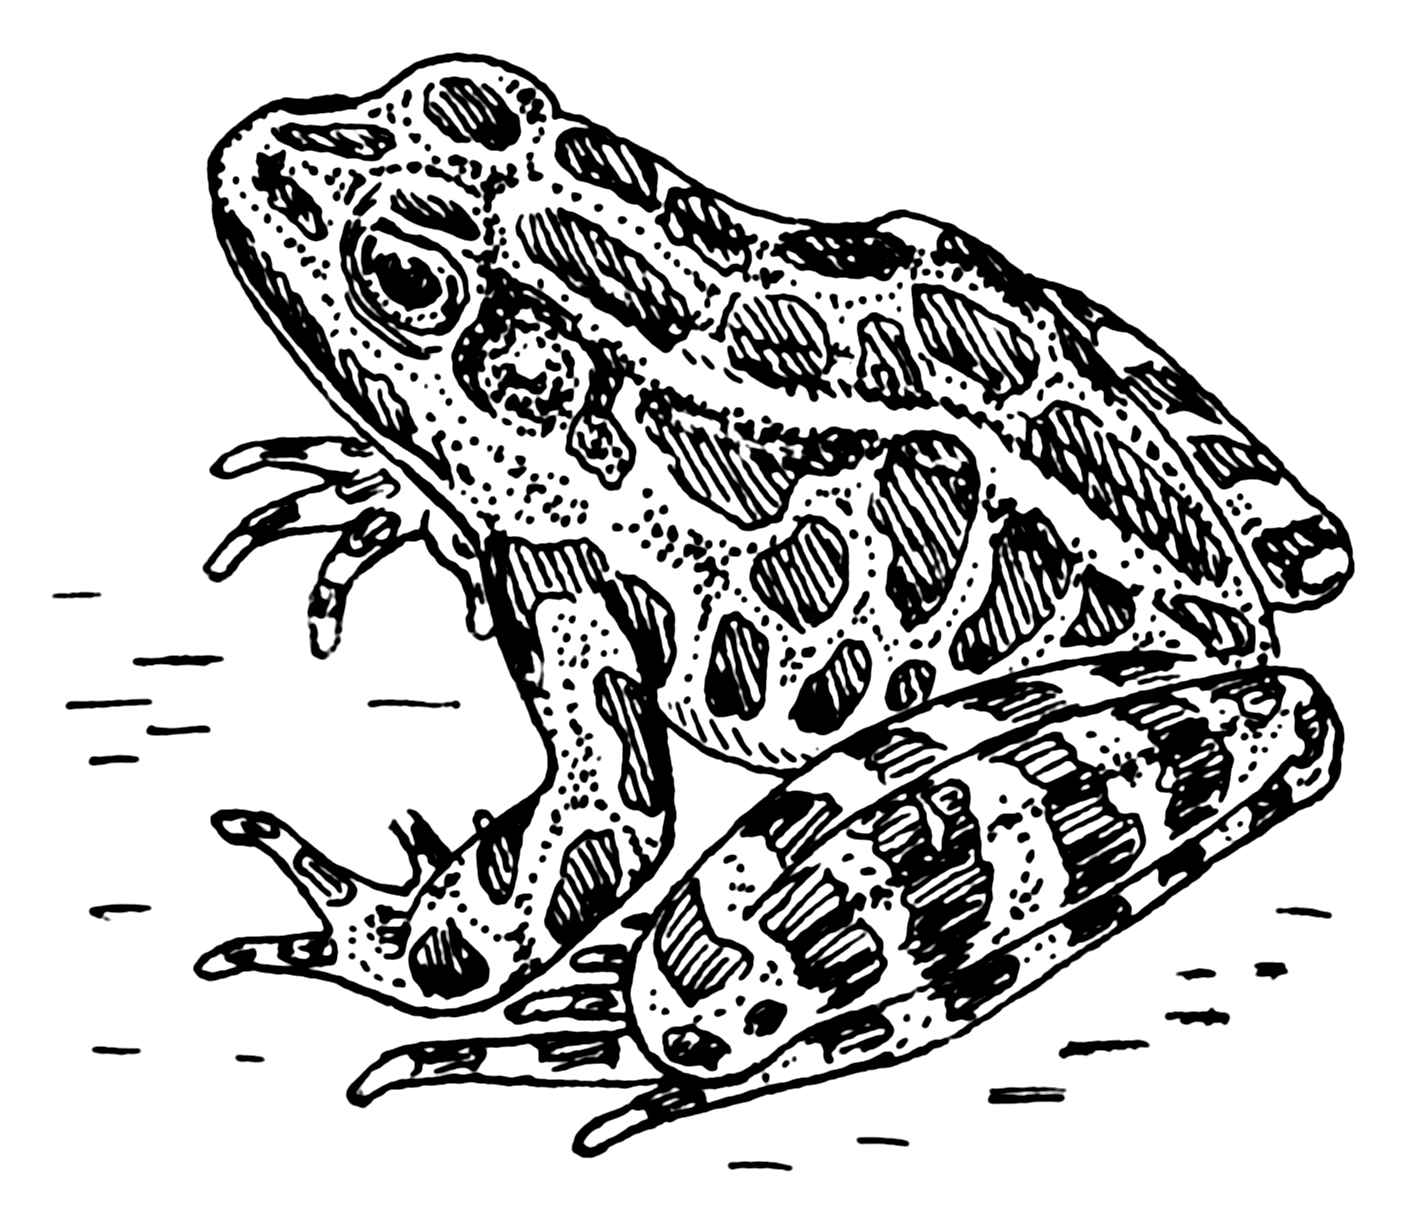
\includegraphics[scale=1]{img/Frog_(PSF).png}
           
        \end{figure}
        
        \Huge
        \textbf{\textsc{Egzamin licencjacki}}
        
        \vspace{0.5cm}
        \Large
        \textsc{Odpowiedzi na pytania} \\ 
        \line(1,0){330}

        \normalsize
        \textit{,,Nigdy nie rozumiałem po co ludzie czytają treści z obiektówki''}
        \vspace{1cm}

        \textit{\textsc{Autorzy}}\\
        \vspace{5mm}
  
        \textbf{\textsc{Dziurawy Ponton} \\ \textsc{Załatany Ponton} \\ \textsc{Puchaty Pompon} \\ \textsc{Zatopiony Ponton} \\ \textsc{Tonący Ponton}\\ \textsc{V} \\ \textsc{Nijaki Ponton} \\ \textsc{Pontus Euxinus}} \\
 
        \vfill

        Kraków \\
        Anno Domini 2024
    \end{center}
\end{titlepage}
\tableofcontents

\section*{Licencja}
    \begin{figure}[h]
    	\begin{minipage}[c]{0.25\textwidth}
    		
\includegraphics[width=0.7\textwidth]{images/licencja.png}
    	\end{minipage}\hfill
    	\begin{minipage}[c]{0.75\textwidth}
    		\caption*{
    			Ten utwór jest dostępny na 
    			\href{https://creativecommons.org/licenses/by-sa/4.0/}{licencji Creative Commons Uznanie autorstwa
    			na tych samych warunkach 4.0 Międzynarodowe.}
    		}
    	\end{minipage}
    \end{figure}
Zawartość rozdziału \ref{sysopy} podchodzi z notatek zadedykowanych domenie publicznej (CC0 1.0); nie jest ona napisana przez wylistowanych (anonimowych) autorów tego opracowania.

% Actual content
\mainmatter

% ROK 1, SEMESTR ZIMOWY
\begin{definition}[Definicja permutacyjna wyznacznika]
Jeśli \(\field\) jest ciałem i \(n \in \natural\), to \textbf{wyznacznikiem} nazwiemy funkcję \(f : \fieldset^{n \times n}\) taką, że:

\[
f(A) = \sum_{\sigma \in S_n} \sgn(\sigma) \cdot A_{1, \; \sigma(1)} \cdot A_{2, \; \sigma(2)} \cdot A_{3, \; \sigma(3)} \cdot \dots \cdot A_{n, \; \sigma(n)} 
\]

gdzie \(A_{ij}\) oznacza komórkę macierzy znajdującą się w \(i\)-tym wierszu i \(j\)-tej kolumnie, a \(S_n\) oznacza zbiór wszystkich permutacji zbioru \(n\)-elementowego.

\end{definition}

\begin{definition}[Definicja ,,objętościowa'' wyznacznika]
Niech \(\field\) będzie ciałem i \(n \in \natural\). Ponadto, niech \(v_1, v_2, v_3, \dots, v_n \in \fieldset^{n}\). Wówczas tuplę \((v_1, v_2, v_3, \dots, v_n) \in (\fieldset^{n})^{n}\) możemy trywialnie utożsamić z macierzą \(M \in \fieldset^{n \times n}\) (i vice versa), poprzez utożsamienie każdego wektora \(\fieldset^{n}\) z pojedynczym wierszem tej macierzy.

Stosując taką notację, mówimy że funkcja \(f: \fieldset^{n \times n} \rightarrow \fieldset\) jest \textbf{wyznacznikiem}, jeśli spełnia następujące warunki: 

\begin{enumerate}
    \item \(f(v_1, v_2, \dots, \lambda v_i, \dots, v_n) = \lambda \cdot f(v_1, v_2, \dots, v_i, \dots, v_n) \)
    \item \(f(v_1, v_2, \dots, v_i + v_{i}', \dots, v_n) = f(v_1, v_2, \dots, v_i, \dots, v_n) + f(v_1, v_2, \dots, v_{i}', \dots, v_n) \)
    \item Jeżeli istnieje takie \(i\), że \(v_i = v_{i+1}\), to \(f(v_1, v_2, \dots, v_i, v_{i+1}, \dots v_n) = 0\)
    \item \(f\) na macierzy identycznościowej przyjmuje wartość \(1\). 
\end{enumerate}

Postulaty te wynikają z chęci stworzenia funkcji obliczającej zorientowaną objętość wielowymiarowego równoległościanu (opisywanego wektorami).

Można wykazać, że dla określonego \(n \in \natural\) istnieje dokładnie 1 funkcja spełniająca wyżej wymienione warunki. Definicja ta okazuje się być równoważna z tą wcześniejszą.

\end{definition}

Wyznacznik oznaczamy jako \(\det\).
\begin{theorem}
Dla dowolnych zbiorów \(A, B, C\) zachodzi
\begin{equation*}
    \pars{A^B}^C \eqnum A^{B \times C}
\end{equation*}
\end{theorem}
\begin{proof}
Z~definicji --- konstruujemy bijekcję
\begin{equation*}
    \alpha\colon \pars{A^B}^C \function A^{B \times C}
\end{equation*}
Funkcja \(\alpha\)~przyjmuje funkcję \(C \function A^B\) i~zwraca funkcję \(B \times C \function A\). Zdefiniujmy \(\alpha\)~następująco:
\begin{equation*}
    \begin{split}
        \alpha\pars{f}
            &\coloneqq \pars{\text{taka funkcja \(\gamma\), że \(\gamma\pars{b, c} = \pars{f\pars{c}}\pars{b}\)}}\\
            &\coloneqq \set{\pars{\pars{b, c}, \pars{f\pars{c}}\pars{b}} : \pars{b, c} \in B \times C}
    \end{split}
\end{equation*}
Nadużywając trochę notacji, możemy to bardziej intuicyjnie zapisać jako
\begin{equation*}
    \pars{\alpha\pars{f}}\pars{b, c} \coloneqq \pars{f\pars{c}}\pars{b}
\end{equation*}
Musimy pokazać, że \(\alpha\)~bijekcją.
\begin{description}
    \item[Injektywność.] Weźmy różne \(f_1, f_2 \in \pars{A^B}^C\) i~pokażmy, że \(\alpha\pars{f_1} \neq \alpha\pars{f_2}\).

        Co to znaczy, że \(f_1, f_2\) są różne? To są funkcje \(C \function A^B\), więc gdy są różne, to na jakimś argumencie \(c_0 \in C\) przyjmują różne wartości:
        \begin{equation*}
            f_1\pars{c_0} \neq f_2\pars{c_0}
        \end{equation*}
        Ale to też są funkcje, tym razem \(B \function A\). Czyli skoro są różne, to na pewnym argumencie \(b_0 \in B\) przyjmują różne wartości:
        \begin{equation*}
            \pars{f_1\pars{c_0}}\pars{b_0} \neq \pars{f_2\pars{c_0}}\pars{b_0}
        \end{equation*}
        Możemy to zapisać za pomocą \(\alpha\)~jako
        \begin{equation*}
            \pars{\alpha\pars{f_1}}\pars{b_0, c_0} \neq \pars{\alpha\pars{f_2}}\pars{b_0, c_0}
        \end{equation*}
        Oznacza to, że funkcje \(\alpha\pars{f_1}, \alpha\pars{f_2}\colon B \times C \function \alpha\) przyjmują różne wartości na argumencie \(\pars{b_0, c_0} \in B \times C\). A~zatem są to różne funkcje \(\alpha\pars{f_1} \neq \alpha\pars{f_2}\), co właśnie chcieliśmy udowodnić.
    \item[Surjektywność.] Weźmy \(g \in A^{B \times C}\). Musimy pokazać, że istnieje \(f \in \pars{A^B}^C\) takie, że
        \begin{equation*}
            \alpha\pars{f} = g
        \end{equation*}
        Niewątpliwie, w~dziedzinie funkcji \(\alpha\)~znajduje się w~szczególności \(f_0\colon C \function A^B\)~zdefiniowane następująco
        \begin{equation*}
            \begin{split}
                f_0\pars{c}
                    &\coloneqq \pars{\text{taka funkcja \(\gamma\), że \(\gamma\pars{b} = g\pars{b, c}\)}}\\
                    &\coloneqq \set{\pars{b, g\pars{b, c}} : b \in B}
            \end{split}
        \end{equation*}
        co można, ponownie z~drobnym nadużyciem notacji można zapisać jako
        \begin{equation*}
            \pars{f_0\pars{c}}\pars{b} \coloneqq g\pars{b, c}
        \end{equation*}
        Zobaczmy, że dla dowolnej pary \(\pars{b_0, c_0} \in B \times C\) zachodzi
        \begin{align*}
            \pars{\alpha\pars{f_0}}\pars{b_0, c_0}
                &= \pars{f_0\pars{c_0}}\pars{b_0} && \text{z~definicji \(\alpha\)}\\
                &= g\pars{b_0, c_0} && \text{z~definicji \(f_0\)}
        \end{align*}
        Zatem istotnie \(\alpha\pars{f_0} = g\) jako funkcje.
\end{description}
\end{proof}
\begin{theorem}
Dla dowolnych zbiorów \(A, B, C\) zachodzi
\begin{equation*}
    \pars{A \times B}^C \eqnum A^C \times B^C
\end{equation*}
\end{theorem}
\begin{proof}
Korzystamy z~przemienności i~konstruujemy bijekcję
\begin{equation*}
    \alpha\colon A^C \times B^C \function \pars{A \times B}^C
\end{equation*}
Funkcja \(\alpha\)~przyjmuje parę funkcji \(\pars{C \function A, C \function B}\) i~zwraca funkcję \(C \function A \times B\). Definiujemy ją następująco:
\begin{equation*}
    \begin{split}
        \alpha\pars{f, g}
            &\coloneqq \pars{\text{taka funkcja \(\eta\), że \(\eta\pars{c} = \pars{f\pars{c}, g\pars{c}}\)}}\\
            &\coloneqq \set{\pars{c, \pars{f\pars{c}, g\pars{c}}} : c \in C}
    \end{split}
\end{equation*}
Inaczej:
\begin{equation*}
    \pars{\alpha\pars{f, g}}\pars{c} = \pars{f\pars{c}, g\pars{c}}
\end{equation*}
Musimy pokazać, że \(\alpha\)~jest bijekcją.
\begin{description}
    \item[Injektywność.] Weźmy różne pary \(\pars{f_1, g_1}, \pars{f_2, g_2} \in A^C \times B^C\). Skoro są to różne pary funkcji, to istnieje takie \(c_0 \in C\), że \(f_1\pars{c_0} \neq f_2\pars{c_0}\) lub istnieje takie \(c_0' \in C\), że \(g_1\pars{c_0'} \neq g_2\pars{c_0'}\). Bez straty ogólności, przyjmijmy pierwszą opcję. Widzimy, że
    \begin{equation*}
        \pars{\alpha\pars{f_1, g_1}}\pars{c_0} = \pars{f_1\pars{c_0}, g_1\pars{c_0}} \neq \pars{f_2\pars{c_0}, g_2\pars{c_0}} = \pars{\alpha\pars{f_2, g_2}}\pars{c_0}
    \end{equation*}
    Oznacza to, że \(\alpha\pars{f_1, g_1}\) i~\(\alpha\pars{f_2, g_2}\) są różnymi funkcjami --- tak, jak chcieliśmy.
    \item[Surjektywność.] Weźmy \(h \in \pars{A \times B}^C\). Musimy pokazać, że istnieje para \(\pars{f_0, g_0} \in A^C \times B^C\) taka, że
        \begin{equation*}
            \alpha\pars{f_0, g_0} = h
        \end{equation*}
        Weźmy
        \begin{gather*}
            f_0\colon C \function A\\
            f_0\pars{c} \coloneqq \text{lewy element pary \(h\pars{c}\)}
        \end{gather*}
        oraz
        \begin{gather*}
            g_0\colon C \function B\\
            g_0\pars{c} \coloneqq \text{prawy element pary \(h\pars{c}\)}
        \end{gather*}
        Teraz dla dowolnego \(c_0 \in C\) mamy
        \begin{equation*}
            \pars{\alpha\pars{f_0, g_0}}\pars{c_0}
                = \pars{f_0\pars{c_0}, g_0\pars{c_0}}
                = \pars{\text{lewy z~\(h\pars{c_0}\)}, \text{prawy z~\(h\pars{c_0}\)}}
                = h\pars{c_0}
        \end{equation*}
        co dowodzi, że \(\alpha\pars{f_0, g_0} = h\) jako funkcje.
        
        Jako bonus możemy zastanowić się, jak teoriomnogościowo wyciągać lewy i~prawy element pary uporządkowanej. Wykorzystamy definicję \ref{mfi:cartesian_and_relations:cartesian_definitions:def:ordered_pair}.
        \begin{itemize}
            \item \(\bigcup\bigcap p\) jest lewym elementem pary \(p\)
                \begin{equation*}
                    p = \pars{a, b} = \set{\set{a}, \set{a, b}} \overset{\bigcap}{\longrightarrow} \set{a} \overset{\bigcup}{\longrightarrow} a
                \end{equation*}
            \item \(\bigcup\pars{\bigcup p \setminus \bigcap p}\) jest prawym elementem pary \(p\)
                \begin{equation*}
                    p = \pars{a, b} = \set{\set{a}, \set{a, b}} \overset{\bigcap}{\longrightarrow} \set{a} \overset{\bigcup \setminus \pars{\mathord{\cdot}}}{\longrightarrow} \set{a, b} \setminus \set{a} = \set{b} \overset{\bigcup}{\longrightarrow} b
                \end{equation*}
        \end{itemize}
\end{description}
\end{proof}


\begin{definition}[Definicja permutacyjna wyznacznika]
Jeśli \(\field\) jest ciałem i \(n \in \natural\), to \textbf{wyznacznikiem} nazwiemy funkcję \(f : \fieldset^{n \times n}\) taką, że:

\[
f(A) = \sum_{\sigma \in S_n} \sgn(\sigma) \cdot A_{1, \; \sigma(1)} \cdot A_{2, \; \sigma(2)} \cdot A_{3, \; \sigma(3)} \cdot \dots \cdot A_{n, \; \sigma(n)} 
\]

gdzie \(A_{ij}\) oznacza komórkę macierzy znajdującą się w \(i\)-tym wierszu i \(j\)-tej kolumnie, a \(S_n\) oznacza zbiór wszystkich permutacji zbioru \(n\)-elementowego.

\end{definition}

\begin{definition}[Definicja ,,objętościowa'' wyznacznika]
Niech \(\field\) będzie ciałem i \(n \in \natural\). Ponadto, niech \(v_1, v_2, v_3, \dots, v_n \in \fieldset^{n}\). Wówczas tuplę \((v_1, v_2, v_3, \dots, v_n) \in (\fieldset^{n})^{n}\) możemy trywialnie utożsamić z macierzą \(M \in \fieldset^{n \times n}\) (i vice versa), poprzez utożsamienie każdego wektora \(\fieldset^{n}\) z pojedynczym wierszem tej macierzy.

Stosując taką notację, mówimy że funkcja \(f: \fieldset^{n \times n} \rightarrow \fieldset\) jest \textbf{wyznacznikiem}, jeśli spełnia następujące warunki: 

\begin{enumerate}
    \item \(f(v_1, v_2, \dots, \lambda v_i, \dots, v_n) = \lambda \cdot f(v_1, v_2, \dots, v_i, \dots, v_n) \)
    \item \(f(v_1, v_2, \dots, v_i + v_{i}', \dots, v_n) = f(v_1, v_2, \dots, v_i, \dots, v_n) + f(v_1, v_2, \dots, v_{i}', \dots, v_n) \)
    \item Jeżeli istnieje takie \(i\), że \(v_i = v_{i+1}\), to \(f(v_1, v_2, \dots, v_i, v_{i+1}, \dots v_n) = 0\)
    \item \(f\) na macierzy identycznościowej przyjmuje wartość \(1\). 
\end{enumerate}

Postulaty te wynikają z chęci stworzenia funkcji obliczającej zorientowaną objętość wielowymiarowego równoległościanu (opisywanego wektorami).

Można wykazać, że dla określonego \(n \in \natural\) istnieje dokładnie 1 funkcja spełniająca wyżej wymienione warunki. Definicja ta okazuje się być równoważna z tą wcześniejszą.

\end{definition}

Wyznacznik oznaczamy jako \(\det\).
\begin{theorem}
Dla dowolnych zbiorów \(A, B, C\) zachodzi
\begin{equation*}
    \pars{A^B}^C \eqnum A^{B \times C}
\end{equation*}
\end{theorem}
\begin{proof}
Z~definicji --- konstruujemy bijekcję
\begin{equation*}
    \alpha\colon \pars{A^B}^C \function A^{B \times C}
\end{equation*}
Funkcja \(\alpha\)~przyjmuje funkcję \(C \function A^B\) i~zwraca funkcję \(B \times C \function A\). Zdefiniujmy \(\alpha\)~następująco:
\begin{equation*}
    \begin{split}
        \alpha\pars{f}
            &\coloneqq \pars{\text{taka funkcja \(\gamma\), że \(\gamma\pars{b, c} = \pars{f\pars{c}}\pars{b}\)}}\\
            &\coloneqq \set{\pars{\pars{b, c}, \pars{f\pars{c}}\pars{b}} : \pars{b, c} \in B \times C}
    \end{split}
\end{equation*}
Nadużywając trochę notacji, możemy to bardziej intuicyjnie zapisać jako
\begin{equation*}
    \pars{\alpha\pars{f}}\pars{b, c} \coloneqq \pars{f\pars{c}}\pars{b}
\end{equation*}
Musimy pokazać, że \(\alpha\)~bijekcją.
\begin{description}
    \item[Injektywność.] Weźmy różne \(f_1, f_2 \in \pars{A^B}^C\) i~pokażmy, że \(\alpha\pars{f_1} \neq \alpha\pars{f_2}\).

        Co to znaczy, że \(f_1, f_2\) są różne? To są funkcje \(C \function A^B\), więc gdy są różne, to na jakimś argumencie \(c_0 \in C\) przyjmują różne wartości:
        \begin{equation*}
            f_1\pars{c_0} \neq f_2\pars{c_0}
        \end{equation*}
        Ale to też są funkcje, tym razem \(B \function A\). Czyli skoro są różne, to na pewnym argumencie \(b_0 \in B\) przyjmują różne wartości:
        \begin{equation*}
            \pars{f_1\pars{c_0}}\pars{b_0} \neq \pars{f_2\pars{c_0}}\pars{b_0}
        \end{equation*}
        Możemy to zapisać za pomocą \(\alpha\)~jako
        \begin{equation*}
            \pars{\alpha\pars{f_1}}\pars{b_0, c_0} \neq \pars{\alpha\pars{f_2}}\pars{b_0, c_0}
        \end{equation*}
        Oznacza to, że funkcje \(\alpha\pars{f_1}, \alpha\pars{f_2}\colon B \times C \function \alpha\) przyjmują różne wartości na argumencie \(\pars{b_0, c_0} \in B \times C\). A~zatem są to różne funkcje \(\alpha\pars{f_1} \neq \alpha\pars{f_2}\), co właśnie chcieliśmy udowodnić.
    \item[Surjektywność.] Weźmy \(g \in A^{B \times C}\). Musimy pokazać, że istnieje \(f \in \pars{A^B}^C\) takie, że
        \begin{equation*}
            \alpha\pars{f} = g
        \end{equation*}
        Niewątpliwie, w~dziedzinie funkcji \(\alpha\)~znajduje się w~szczególności \(f_0\colon C \function A^B\)~zdefiniowane następująco
        \begin{equation*}
            \begin{split}
                f_0\pars{c}
                    &\coloneqq \pars{\text{taka funkcja \(\gamma\), że \(\gamma\pars{b} = g\pars{b, c}\)}}\\
                    &\coloneqq \set{\pars{b, g\pars{b, c}} : b \in B}
            \end{split}
        \end{equation*}
        co można, ponownie z~drobnym nadużyciem notacji można zapisać jako
        \begin{equation*}
            \pars{f_0\pars{c}}\pars{b} \coloneqq g\pars{b, c}
        \end{equation*}
        Zobaczmy, że dla dowolnej pary \(\pars{b_0, c_0} \in B \times C\) zachodzi
        \begin{align*}
            \pars{\alpha\pars{f_0}}\pars{b_0, c_0}
                &= \pars{f_0\pars{c_0}}\pars{b_0} && \text{z~definicji \(\alpha\)}\\
                &= g\pars{b_0, c_0} && \text{z~definicji \(f_0\)}
        \end{align*}
        Zatem istotnie \(\alpha\pars{f_0} = g\) jako funkcje.
\end{description}
\end{proof}
\begin{theorem}
Dla dowolnych zbiorów \(A, B, C\) zachodzi
\begin{equation*}
    \pars{A \times B}^C \eqnum A^C \times B^C
\end{equation*}
\end{theorem}
\begin{proof}
Korzystamy z~przemienności i~konstruujemy bijekcję
\begin{equation*}
    \alpha\colon A^C \times B^C \function \pars{A \times B}^C
\end{equation*}
Funkcja \(\alpha\)~przyjmuje parę funkcji \(\pars{C \function A, C \function B}\) i~zwraca funkcję \(C \function A \times B\). Definiujemy ją następująco:
\begin{equation*}
    \begin{split}
        \alpha\pars{f, g}
            &\coloneqq \pars{\text{taka funkcja \(\eta\), że \(\eta\pars{c} = \pars{f\pars{c}, g\pars{c}}\)}}\\
            &\coloneqq \set{\pars{c, \pars{f\pars{c}, g\pars{c}}} : c \in C}
    \end{split}
\end{equation*}
Inaczej:
\begin{equation*}
    \pars{\alpha\pars{f, g}}\pars{c} = \pars{f\pars{c}, g\pars{c}}
\end{equation*}
Musimy pokazać, że \(\alpha\)~jest bijekcją.
\begin{description}
    \item[Injektywność.] Weźmy różne pary \(\pars{f_1, g_1}, \pars{f_2, g_2} \in A^C \times B^C\). Skoro są to różne pary funkcji, to istnieje takie \(c_0 \in C\), że \(f_1\pars{c_0} \neq f_2\pars{c_0}\) lub istnieje takie \(c_0' \in C\), że \(g_1\pars{c_0'} \neq g_2\pars{c_0'}\). Bez straty ogólności, przyjmijmy pierwszą opcję. Widzimy, że
    \begin{equation*}
        \pars{\alpha\pars{f_1, g_1}}\pars{c_0} = \pars{f_1\pars{c_0}, g_1\pars{c_0}} \neq \pars{f_2\pars{c_0}, g_2\pars{c_0}} = \pars{\alpha\pars{f_2, g_2}}\pars{c_0}
    \end{equation*}
    Oznacza to, że \(\alpha\pars{f_1, g_1}\) i~\(\alpha\pars{f_2, g_2}\) są różnymi funkcjami --- tak, jak chcieliśmy.
    \item[Surjektywność.] Weźmy \(h \in \pars{A \times B}^C\). Musimy pokazać, że istnieje para \(\pars{f_0, g_0} \in A^C \times B^C\) taka, że
        \begin{equation*}
            \alpha\pars{f_0, g_0} = h
        \end{equation*}
        Weźmy
        \begin{gather*}
            f_0\colon C \function A\\
            f_0\pars{c} \coloneqq \text{lewy element pary \(h\pars{c}\)}
        \end{gather*}
        oraz
        \begin{gather*}
            g_0\colon C \function B\\
            g_0\pars{c} \coloneqq \text{prawy element pary \(h\pars{c}\)}
        \end{gather*}
        Teraz dla dowolnego \(c_0 \in C\) mamy
        \begin{equation*}
            \pars{\alpha\pars{f_0, g_0}}\pars{c_0}
                = \pars{f_0\pars{c_0}, g_0\pars{c_0}}
                = \pars{\text{lewy z~\(h\pars{c_0}\)}, \text{prawy z~\(h\pars{c_0}\)}}
                = h\pars{c_0}
        \end{equation*}
        co dowodzi, że \(\alpha\pars{f_0, g_0} = h\) jako funkcje.
        
        Jako bonus możemy zastanowić się, jak teoriomnogościowo wyciągać lewy i~prawy element pary uporządkowanej. Wykorzystamy definicję \ref{mfi:cartesian_and_relations:cartesian_definitions:def:ordered_pair}.
        \begin{itemize}
            \item \(\bigcup\bigcap p\) jest lewym elementem pary \(p\)
                \begin{equation*}
                    p = \pars{a, b} = \set{\set{a}, \set{a, b}} \overset{\bigcap}{\longrightarrow} \set{a} \overset{\bigcup}{\longrightarrow} a
                \end{equation*}
            \item \(\bigcup\pars{\bigcup p \setminus \bigcap p}\) jest prawym elementem pary \(p\)
                \begin{equation*}
                    p = \pars{a, b} = \set{\set{a}, \set{a, b}} \overset{\bigcap}{\longrightarrow} \set{a} \overset{\bigcup \setminus \pars{\mathord{\cdot}}}{\longrightarrow} \set{a, b} \setminus \set{a} = \set{b} \overset{\bigcup}{\longrightarrow} b
                \end{equation*}
        \end{itemize}
\end{description}
\end{proof}


\begin{definition}[Definicja permutacyjna wyznacznika]
Jeśli \(\field\) jest ciałem i \(n \in \natural\), to \textbf{wyznacznikiem} nazwiemy funkcję \(f : \fieldset^{n \times n}\) taką, że:

\[
f(A) = \sum_{\sigma \in S_n} \sgn(\sigma) \cdot A_{1, \; \sigma(1)} \cdot A_{2, \; \sigma(2)} \cdot A_{3, \; \sigma(3)} \cdot \dots \cdot A_{n, \; \sigma(n)} 
\]

gdzie \(A_{ij}\) oznacza komórkę macierzy znajdującą się w \(i\)-tym wierszu i \(j\)-tej kolumnie, a \(S_n\) oznacza zbiór wszystkich permutacji zbioru \(n\)-elementowego.

\end{definition}

\begin{definition}[Definicja ,,objętościowa'' wyznacznika]
Niech \(\field\) będzie ciałem i \(n \in \natural\). Ponadto, niech \(v_1, v_2, v_3, \dots, v_n \in \fieldset^{n}\). Wówczas tuplę \((v_1, v_2, v_3, \dots, v_n) \in (\fieldset^{n})^{n}\) możemy trywialnie utożsamić z macierzą \(M \in \fieldset^{n \times n}\) (i vice versa), poprzez utożsamienie każdego wektora \(\fieldset^{n}\) z pojedynczym wierszem tej macierzy.

Stosując taką notację, mówimy że funkcja \(f: \fieldset^{n \times n} \rightarrow \fieldset\) jest \textbf{wyznacznikiem}, jeśli spełnia następujące warunki: 

\begin{enumerate}
    \item \(f(v_1, v_2, \dots, \lambda v_i, \dots, v_n) = \lambda \cdot f(v_1, v_2, \dots, v_i, \dots, v_n) \)
    \item \(f(v_1, v_2, \dots, v_i + v_{i}', \dots, v_n) = f(v_1, v_2, \dots, v_i, \dots, v_n) + f(v_1, v_2, \dots, v_{i}', \dots, v_n) \)
    \item Jeżeli istnieje takie \(i\), że \(v_i = v_{i+1}\), to \(f(v_1, v_2, \dots, v_i, v_{i+1}, \dots v_n) = 0\)
    \item \(f\) na macierzy identycznościowej przyjmuje wartość \(1\). 
\end{enumerate}

Postulaty te wynikają z chęci stworzenia funkcji obliczającej zorientowaną objętość wielowymiarowego równoległościanu (opisywanego wektorami).

Można wykazać, że dla określonego \(n \in \natural\) istnieje dokładnie 1 funkcja spełniająca wyżej wymienione warunki. Definicja ta okazuje się być równoważna z tą wcześniejszą.

\end{definition}

Wyznacznik oznaczamy jako \(\det\).
\begin{theorem}
Dla dowolnych zbiorów \(A, B, C\) zachodzi
\begin{equation*}
    \pars{A^B}^C \eqnum A^{B \times C}
\end{equation*}
\end{theorem}
\begin{proof}
Z~definicji --- konstruujemy bijekcję
\begin{equation*}
    \alpha\colon \pars{A^B}^C \function A^{B \times C}
\end{equation*}
Funkcja \(\alpha\)~przyjmuje funkcję \(C \function A^B\) i~zwraca funkcję \(B \times C \function A\). Zdefiniujmy \(\alpha\)~następująco:
\begin{equation*}
    \begin{split}
        \alpha\pars{f}
            &\coloneqq \pars{\text{taka funkcja \(\gamma\), że \(\gamma\pars{b, c} = \pars{f\pars{c}}\pars{b}\)}}\\
            &\coloneqq \set{\pars{\pars{b, c}, \pars{f\pars{c}}\pars{b}} : \pars{b, c} \in B \times C}
    \end{split}
\end{equation*}
Nadużywając trochę notacji, możemy to bardziej intuicyjnie zapisać jako
\begin{equation*}
    \pars{\alpha\pars{f}}\pars{b, c} \coloneqq \pars{f\pars{c}}\pars{b}
\end{equation*}
Musimy pokazać, że \(\alpha\)~bijekcją.
\begin{description}
    \item[Injektywność.] Weźmy różne \(f_1, f_2 \in \pars{A^B}^C\) i~pokażmy, że \(\alpha\pars{f_1} \neq \alpha\pars{f_2}\).

        Co to znaczy, że \(f_1, f_2\) są różne? To są funkcje \(C \function A^B\), więc gdy są różne, to na jakimś argumencie \(c_0 \in C\) przyjmują różne wartości:
        \begin{equation*}
            f_1\pars{c_0} \neq f_2\pars{c_0}
        \end{equation*}
        Ale to też są funkcje, tym razem \(B \function A\). Czyli skoro są różne, to na pewnym argumencie \(b_0 \in B\) przyjmują różne wartości:
        \begin{equation*}
            \pars{f_1\pars{c_0}}\pars{b_0} \neq \pars{f_2\pars{c_0}}\pars{b_0}
        \end{equation*}
        Możemy to zapisać za pomocą \(\alpha\)~jako
        \begin{equation*}
            \pars{\alpha\pars{f_1}}\pars{b_0, c_0} \neq \pars{\alpha\pars{f_2}}\pars{b_0, c_0}
        \end{equation*}
        Oznacza to, że funkcje \(\alpha\pars{f_1}, \alpha\pars{f_2}\colon B \times C \function \alpha\) przyjmują różne wartości na argumencie \(\pars{b_0, c_0} \in B \times C\). A~zatem są to różne funkcje \(\alpha\pars{f_1} \neq \alpha\pars{f_2}\), co właśnie chcieliśmy udowodnić.
    \item[Surjektywność.] Weźmy \(g \in A^{B \times C}\). Musimy pokazać, że istnieje \(f \in \pars{A^B}^C\) takie, że
        \begin{equation*}
            \alpha\pars{f} = g
        \end{equation*}
        Niewątpliwie, w~dziedzinie funkcji \(\alpha\)~znajduje się w~szczególności \(f_0\colon C \function A^B\)~zdefiniowane następująco
        \begin{equation*}
            \begin{split}
                f_0\pars{c}
                    &\coloneqq \pars{\text{taka funkcja \(\gamma\), że \(\gamma\pars{b} = g\pars{b, c}\)}}\\
                    &\coloneqq \set{\pars{b, g\pars{b, c}} : b \in B}
            \end{split}
        \end{equation*}
        co można, ponownie z~drobnym nadużyciem notacji można zapisać jako
        \begin{equation*}
            \pars{f_0\pars{c}}\pars{b} \coloneqq g\pars{b, c}
        \end{equation*}
        Zobaczmy, że dla dowolnej pary \(\pars{b_0, c_0} \in B \times C\) zachodzi
        \begin{align*}
            \pars{\alpha\pars{f_0}}\pars{b_0, c_0}
                &= \pars{f_0\pars{c_0}}\pars{b_0} && \text{z~definicji \(\alpha\)}\\
                &= g\pars{b_0, c_0} && \text{z~definicji \(f_0\)}
        \end{align*}
        Zatem istotnie \(\alpha\pars{f_0} = g\) jako funkcje.
\end{description}
\end{proof}
\begin{theorem}
Dla dowolnych zbiorów \(A, B, C\) zachodzi
\begin{equation*}
    \pars{A \times B}^C \eqnum A^C \times B^C
\end{equation*}
\end{theorem}
\begin{proof}
Korzystamy z~przemienności i~konstruujemy bijekcję
\begin{equation*}
    \alpha\colon A^C \times B^C \function \pars{A \times B}^C
\end{equation*}
Funkcja \(\alpha\)~przyjmuje parę funkcji \(\pars{C \function A, C \function B}\) i~zwraca funkcję \(C \function A \times B\). Definiujemy ją następująco:
\begin{equation*}
    \begin{split}
        \alpha\pars{f, g}
            &\coloneqq \pars{\text{taka funkcja \(\eta\), że \(\eta\pars{c} = \pars{f\pars{c}, g\pars{c}}\)}}\\
            &\coloneqq \set{\pars{c, \pars{f\pars{c}, g\pars{c}}} : c \in C}
    \end{split}
\end{equation*}
Inaczej:
\begin{equation*}
    \pars{\alpha\pars{f, g}}\pars{c} = \pars{f\pars{c}, g\pars{c}}
\end{equation*}
Musimy pokazać, że \(\alpha\)~jest bijekcją.
\begin{description}
    \item[Injektywność.] Weźmy różne pary \(\pars{f_1, g_1}, \pars{f_2, g_2} \in A^C \times B^C\). Skoro są to różne pary funkcji, to istnieje takie \(c_0 \in C\), że \(f_1\pars{c_0} \neq f_2\pars{c_0}\) lub istnieje takie \(c_0' \in C\), że \(g_1\pars{c_0'} \neq g_2\pars{c_0'}\). Bez straty ogólności, przyjmijmy pierwszą opcję. Widzimy, że
    \begin{equation*}
        \pars{\alpha\pars{f_1, g_1}}\pars{c_0} = \pars{f_1\pars{c_0}, g_1\pars{c_0}} \neq \pars{f_2\pars{c_0}, g_2\pars{c_0}} = \pars{\alpha\pars{f_2, g_2}}\pars{c_0}
    \end{equation*}
    Oznacza to, że \(\alpha\pars{f_1, g_1}\) i~\(\alpha\pars{f_2, g_2}\) są różnymi funkcjami --- tak, jak chcieliśmy.
    \item[Surjektywność.] Weźmy \(h \in \pars{A \times B}^C\). Musimy pokazać, że istnieje para \(\pars{f_0, g_0} \in A^C \times B^C\) taka, że
        \begin{equation*}
            \alpha\pars{f_0, g_0} = h
        \end{equation*}
        Weźmy
        \begin{gather*}
            f_0\colon C \function A\\
            f_0\pars{c} \coloneqq \text{lewy element pary \(h\pars{c}\)}
        \end{gather*}
        oraz
        \begin{gather*}
            g_0\colon C \function B\\
            g_0\pars{c} \coloneqq \text{prawy element pary \(h\pars{c}\)}
        \end{gather*}
        Teraz dla dowolnego \(c_0 \in C\) mamy
        \begin{equation*}
            \pars{\alpha\pars{f_0, g_0}}\pars{c_0}
                = \pars{f_0\pars{c_0}, g_0\pars{c_0}}
                = \pars{\text{lewy z~\(h\pars{c_0}\)}, \text{prawy z~\(h\pars{c_0}\)}}
                = h\pars{c_0}
        \end{equation*}
        co dowodzi, że \(\alpha\pars{f_0, g_0} = h\) jako funkcje.
        
        Jako bonus możemy zastanowić się, jak teoriomnogościowo wyciągać lewy i~prawy element pary uporządkowanej. Wykorzystamy definicję \ref{mfi:cartesian_and_relations:cartesian_definitions:def:ordered_pair}.
        \begin{itemize}
            \item \(\bigcup\bigcap p\) jest lewym elementem pary \(p\)
                \begin{equation*}
                    p = \pars{a, b} = \set{\set{a}, \set{a, b}} \overset{\bigcap}{\longrightarrow} \set{a} \overset{\bigcup}{\longrightarrow} a
                \end{equation*}
            \item \(\bigcup\pars{\bigcup p \setminus \bigcap p}\) jest prawym elementem pary \(p\)
                \begin{equation*}
                    p = \pars{a, b} = \set{\set{a}, \set{a, b}} \overset{\bigcap}{\longrightarrow} \set{a} \overset{\bigcup \setminus \pars{\mathord{\cdot}}}{\longrightarrow} \set{a, b} \setminus \set{a} = \set{b} \overset{\bigcup}{\longrightarrow} b
                \end{equation*}
        \end{itemize}
\end{description}
\end{proof}


%\begin{definition}[Definicja permutacyjna wyznacznika]
Jeśli \(\field\) jest ciałem i \(n \in \natural\), to \textbf{wyznacznikiem} nazwiemy funkcję \(f : \fieldset^{n \times n}\) taką, że:

\[
f(A) = \sum_{\sigma \in S_n} \sgn(\sigma) \cdot A_{1, \; \sigma(1)} \cdot A_{2, \; \sigma(2)} \cdot A_{3, \; \sigma(3)} \cdot \dots \cdot A_{n, \; \sigma(n)} 
\]

gdzie \(A_{ij}\) oznacza komórkę macierzy znajdującą się w \(i\)-tym wierszu i \(j\)-tej kolumnie, a \(S_n\) oznacza zbiór wszystkich permutacji zbioru \(n\)-elementowego.

\end{definition}

\begin{definition}[Definicja ,,objętościowa'' wyznacznika]
Niech \(\field\) będzie ciałem i \(n \in \natural\). Ponadto, niech \(v_1, v_2, v_3, \dots, v_n \in \fieldset^{n}\). Wówczas tuplę \((v_1, v_2, v_3, \dots, v_n) \in (\fieldset^{n})^{n}\) możemy trywialnie utożsamić z macierzą \(M \in \fieldset^{n \times n}\) (i vice versa), poprzez utożsamienie każdego wektora \(\fieldset^{n}\) z pojedynczym wierszem tej macierzy.

Stosując taką notację, mówimy że funkcja \(f: \fieldset^{n \times n} \rightarrow \fieldset\) jest \textbf{wyznacznikiem}, jeśli spełnia następujące warunki: 

\begin{enumerate}
    \item \(f(v_1, v_2, \dots, \lambda v_i, \dots, v_n) = \lambda \cdot f(v_1, v_2, \dots, v_i, \dots, v_n) \)
    \item \(f(v_1, v_2, \dots, v_i + v_{i}', \dots, v_n) = f(v_1, v_2, \dots, v_i, \dots, v_n) + f(v_1, v_2, \dots, v_{i}', \dots, v_n) \)
    \item Jeżeli istnieje takie \(i\), że \(v_i = v_{i+1}\), to \(f(v_1, v_2, \dots, v_i, v_{i+1}, \dots v_n) = 0\)
    \item \(f\) na macierzy identycznościowej przyjmuje wartość \(1\). 
\end{enumerate}

Postulaty te wynikają z chęci stworzenia funkcji obliczającej zorientowaną objętość wielowymiarowego równoległościanu (opisywanego wektorami).

Można wykazać, że dla określonego \(n \in \natural\) istnieje dokładnie 1 funkcja spełniająca wyżej wymienione warunki. Definicja ta okazuje się być równoważna z tą wcześniejszą.

\end{definition}

Wyznacznik oznaczamy jako \(\det\).
\begin{theorem}
Dla dowolnych zbiorów \(A, B, C\) zachodzi
\begin{equation*}
    \pars{A^B}^C \eqnum A^{B \times C}
\end{equation*}
\end{theorem}
\begin{proof}
Z~definicji --- konstruujemy bijekcję
\begin{equation*}
    \alpha\colon \pars{A^B}^C \function A^{B \times C}
\end{equation*}
Funkcja \(\alpha\)~przyjmuje funkcję \(C \function A^B\) i~zwraca funkcję \(B \times C \function A\). Zdefiniujmy \(\alpha\)~następująco:
\begin{equation*}
    \begin{split}
        \alpha\pars{f}
            &\coloneqq \pars{\text{taka funkcja \(\gamma\), że \(\gamma\pars{b, c} = \pars{f\pars{c}}\pars{b}\)}}\\
            &\coloneqq \set{\pars{\pars{b, c}, \pars{f\pars{c}}\pars{b}} : \pars{b, c} \in B \times C}
    \end{split}
\end{equation*}
Nadużywając trochę notacji, możemy to bardziej intuicyjnie zapisać jako
\begin{equation*}
    \pars{\alpha\pars{f}}\pars{b, c} \coloneqq \pars{f\pars{c}}\pars{b}
\end{equation*}
Musimy pokazać, że \(\alpha\)~bijekcją.
\begin{description}
    \item[Injektywność.] Weźmy różne \(f_1, f_2 \in \pars{A^B}^C\) i~pokażmy, że \(\alpha\pars{f_1} \neq \alpha\pars{f_2}\).

        Co to znaczy, że \(f_1, f_2\) są różne? To są funkcje \(C \function A^B\), więc gdy są różne, to na jakimś argumencie \(c_0 \in C\) przyjmują różne wartości:
        \begin{equation*}
            f_1\pars{c_0} \neq f_2\pars{c_0}
        \end{equation*}
        Ale to też są funkcje, tym razem \(B \function A\). Czyli skoro są różne, to na pewnym argumencie \(b_0 \in B\) przyjmują różne wartości:
        \begin{equation*}
            \pars{f_1\pars{c_0}}\pars{b_0} \neq \pars{f_2\pars{c_0}}\pars{b_0}
        \end{equation*}
        Możemy to zapisać za pomocą \(\alpha\)~jako
        \begin{equation*}
            \pars{\alpha\pars{f_1}}\pars{b_0, c_0} \neq \pars{\alpha\pars{f_2}}\pars{b_0, c_0}
        \end{equation*}
        Oznacza to, że funkcje \(\alpha\pars{f_1}, \alpha\pars{f_2}\colon B \times C \function \alpha\) przyjmują różne wartości na argumencie \(\pars{b_0, c_0} \in B \times C\). A~zatem są to różne funkcje \(\alpha\pars{f_1} \neq \alpha\pars{f_2}\), co właśnie chcieliśmy udowodnić.
    \item[Surjektywność.] Weźmy \(g \in A^{B \times C}\). Musimy pokazać, że istnieje \(f \in \pars{A^B}^C\) takie, że
        \begin{equation*}
            \alpha\pars{f} = g
        \end{equation*}
        Niewątpliwie, w~dziedzinie funkcji \(\alpha\)~znajduje się w~szczególności \(f_0\colon C \function A^B\)~zdefiniowane następująco
        \begin{equation*}
            \begin{split}
                f_0\pars{c}
                    &\coloneqq \pars{\text{taka funkcja \(\gamma\), że \(\gamma\pars{b} = g\pars{b, c}\)}}\\
                    &\coloneqq \set{\pars{b, g\pars{b, c}} : b \in B}
            \end{split}
        \end{equation*}
        co można, ponownie z~drobnym nadużyciem notacji można zapisać jako
        \begin{equation*}
            \pars{f_0\pars{c}}\pars{b} \coloneqq g\pars{b, c}
        \end{equation*}
        Zobaczmy, że dla dowolnej pary \(\pars{b_0, c_0} \in B \times C\) zachodzi
        \begin{align*}
            \pars{\alpha\pars{f_0}}\pars{b_0, c_0}
                &= \pars{f_0\pars{c_0}}\pars{b_0} && \text{z~definicji \(\alpha\)}\\
                &= g\pars{b_0, c_0} && \text{z~definicji \(f_0\)}
        \end{align*}
        Zatem istotnie \(\alpha\pars{f_0} = g\) jako funkcje.
\end{description}
\end{proof}
\begin{theorem}
Dla dowolnych zbiorów \(A, B, C\) zachodzi
\begin{equation*}
    \pars{A \times B}^C \eqnum A^C \times B^C
\end{equation*}
\end{theorem}
\begin{proof}
Korzystamy z~przemienności i~konstruujemy bijekcję
\begin{equation*}
    \alpha\colon A^C \times B^C \function \pars{A \times B}^C
\end{equation*}
Funkcja \(\alpha\)~przyjmuje parę funkcji \(\pars{C \function A, C \function B}\) i~zwraca funkcję \(C \function A \times B\). Definiujemy ją następująco:
\begin{equation*}
    \begin{split}
        \alpha\pars{f, g}
            &\coloneqq \pars{\text{taka funkcja \(\eta\), że \(\eta\pars{c} = \pars{f\pars{c}, g\pars{c}}\)}}\\
            &\coloneqq \set{\pars{c, \pars{f\pars{c}, g\pars{c}}} : c \in C}
    \end{split}
\end{equation*}
Inaczej:
\begin{equation*}
    \pars{\alpha\pars{f, g}}\pars{c} = \pars{f\pars{c}, g\pars{c}}
\end{equation*}
Musimy pokazać, że \(\alpha\)~jest bijekcją.
\begin{description}
    \item[Injektywność.] Weźmy różne pary \(\pars{f_1, g_1}, \pars{f_2, g_2} \in A^C \times B^C\). Skoro są to różne pary funkcji, to istnieje takie \(c_0 \in C\), że \(f_1\pars{c_0} \neq f_2\pars{c_0}\) lub istnieje takie \(c_0' \in C\), że \(g_1\pars{c_0'} \neq g_2\pars{c_0'}\). Bez straty ogólności, przyjmijmy pierwszą opcję. Widzimy, że
    \begin{equation*}
        \pars{\alpha\pars{f_1, g_1}}\pars{c_0} = \pars{f_1\pars{c_0}, g_1\pars{c_0}} \neq \pars{f_2\pars{c_0}, g_2\pars{c_0}} = \pars{\alpha\pars{f_2, g_2}}\pars{c_0}
    \end{equation*}
    Oznacza to, że \(\alpha\pars{f_1, g_1}\) i~\(\alpha\pars{f_2, g_2}\) są różnymi funkcjami --- tak, jak chcieliśmy.
    \item[Surjektywność.] Weźmy \(h \in \pars{A \times B}^C\). Musimy pokazać, że istnieje para \(\pars{f_0, g_0} \in A^C \times B^C\) taka, że
        \begin{equation*}
            \alpha\pars{f_0, g_0} = h
        \end{equation*}
        Weźmy
        \begin{gather*}
            f_0\colon C \function A\\
            f_0\pars{c} \coloneqq \text{lewy element pary \(h\pars{c}\)}
        \end{gather*}
        oraz
        \begin{gather*}
            g_0\colon C \function B\\
            g_0\pars{c} \coloneqq \text{prawy element pary \(h\pars{c}\)}
        \end{gather*}
        Teraz dla dowolnego \(c_0 \in C\) mamy
        \begin{equation*}
            \pars{\alpha\pars{f_0, g_0}}\pars{c_0}
                = \pars{f_0\pars{c_0}, g_0\pars{c_0}}
                = \pars{\text{lewy z~\(h\pars{c_0}\)}, \text{prawy z~\(h\pars{c_0}\)}}
                = h\pars{c_0}
        \end{equation*}
        co dowodzi, że \(\alpha\pars{f_0, g_0} = h\) jako funkcje.
        
        Jako bonus możemy zastanowić się, jak teoriomnogościowo wyciągać lewy i~prawy element pary uporządkowanej. Wykorzystamy definicję \ref{mfi:cartesian_and_relations:cartesian_definitions:def:ordered_pair}.
        \begin{itemize}
            \item \(\bigcup\bigcap p\) jest lewym elementem pary \(p\)
                \begin{equation*}
                    p = \pars{a, b} = \set{\set{a}, \set{a, b}} \overset{\bigcap}{\longrightarrow} \set{a} \overset{\bigcup}{\longrightarrow} a
                \end{equation*}
            \item \(\bigcup\pars{\bigcup p \setminus \bigcap p}\) jest prawym elementem pary \(p\)
                \begin{equation*}
                    p = \pars{a, b} = \set{\set{a}, \set{a, b}} \overset{\bigcap}{\longrightarrow} \set{a} \overset{\bigcup \setminus \pars{\mathord{\cdot}}}{\longrightarrow} \set{a, b} \setminus \set{a} = \set{b} \overset{\bigcup}{\longrightarrow} b
                \end{equation*}
        \end{itemize}
\end{description}
\end{proof}



% ROK 1, SEMESTR LETNI
\begin{definition}[Definicja permutacyjna wyznacznika]
Jeśli \(\field\) jest ciałem i \(n \in \natural\), to \textbf{wyznacznikiem} nazwiemy funkcję \(f : \fieldset^{n \times n}\) taką, że:

\[
f(A) = \sum_{\sigma \in S_n} \sgn(\sigma) \cdot A_{1, \; \sigma(1)} \cdot A_{2, \; \sigma(2)} \cdot A_{3, \; \sigma(3)} \cdot \dots \cdot A_{n, \; \sigma(n)} 
\]

gdzie \(A_{ij}\) oznacza komórkę macierzy znajdującą się w \(i\)-tym wierszu i \(j\)-tej kolumnie, a \(S_n\) oznacza zbiór wszystkich permutacji zbioru \(n\)-elementowego.

\end{definition}

\begin{definition}[Definicja ,,objętościowa'' wyznacznika]
Niech \(\field\) będzie ciałem i \(n \in \natural\). Ponadto, niech \(v_1, v_2, v_3, \dots, v_n \in \fieldset^{n}\). Wówczas tuplę \((v_1, v_2, v_3, \dots, v_n) \in (\fieldset^{n})^{n}\) możemy trywialnie utożsamić z macierzą \(M \in \fieldset^{n \times n}\) (i vice versa), poprzez utożsamienie każdego wektora \(\fieldset^{n}\) z pojedynczym wierszem tej macierzy.

Stosując taką notację, mówimy że funkcja \(f: \fieldset^{n \times n} \rightarrow \fieldset\) jest \textbf{wyznacznikiem}, jeśli spełnia następujące warunki: 

\begin{enumerate}
    \item \(f(v_1, v_2, \dots, \lambda v_i, \dots, v_n) = \lambda \cdot f(v_1, v_2, \dots, v_i, \dots, v_n) \)
    \item \(f(v_1, v_2, \dots, v_i + v_{i}', \dots, v_n) = f(v_1, v_2, \dots, v_i, \dots, v_n) + f(v_1, v_2, \dots, v_{i}', \dots, v_n) \)
    \item Jeżeli istnieje takie \(i\), że \(v_i = v_{i+1}\), to \(f(v_1, v_2, \dots, v_i, v_{i+1}, \dots v_n) = 0\)
    \item \(f\) na macierzy identycznościowej przyjmuje wartość \(1\). 
\end{enumerate}

Postulaty te wynikają z chęci stworzenia funkcji obliczającej zorientowaną objętość wielowymiarowego równoległościanu (opisywanego wektorami).

Można wykazać, że dla określonego \(n \in \natural\) istnieje dokładnie 1 funkcja spełniająca wyżej wymienione warunki. Definicja ta okazuje się być równoważna z tą wcześniejszą.

\end{definition}

Wyznacznik oznaczamy jako \(\det\).
\begin{theorem}
Dla dowolnych zbiorów \(A, B, C\) zachodzi
\begin{equation*}
    \pars{A^B}^C \eqnum A^{B \times C}
\end{equation*}
\end{theorem}
\begin{proof}
Z~definicji --- konstruujemy bijekcję
\begin{equation*}
    \alpha\colon \pars{A^B}^C \function A^{B \times C}
\end{equation*}
Funkcja \(\alpha\)~przyjmuje funkcję \(C \function A^B\) i~zwraca funkcję \(B \times C \function A\). Zdefiniujmy \(\alpha\)~następująco:
\begin{equation*}
    \begin{split}
        \alpha\pars{f}
            &\coloneqq \pars{\text{taka funkcja \(\gamma\), że \(\gamma\pars{b, c} = \pars{f\pars{c}}\pars{b}\)}}\\
            &\coloneqq \set{\pars{\pars{b, c}, \pars{f\pars{c}}\pars{b}} : \pars{b, c} \in B \times C}
    \end{split}
\end{equation*}
Nadużywając trochę notacji, możemy to bardziej intuicyjnie zapisać jako
\begin{equation*}
    \pars{\alpha\pars{f}}\pars{b, c} \coloneqq \pars{f\pars{c}}\pars{b}
\end{equation*}
Musimy pokazać, że \(\alpha\)~bijekcją.
\begin{description}
    \item[Injektywność.] Weźmy różne \(f_1, f_2 \in \pars{A^B}^C\) i~pokażmy, że \(\alpha\pars{f_1} \neq \alpha\pars{f_2}\).

        Co to znaczy, że \(f_1, f_2\) są różne? To są funkcje \(C \function A^B\), więc gdy są różne, to na jakimś argumencie \(c_0 \in C\) przyjmują różne wartości:
        \begin{equation*}
            f_1\pars{c_0} \neq f_2\pars{c_0}
        \end{equation*}
        Ale to też są funkcje, tym razem \(B \function A\). Czyli skoro są różne, to na pewnym argumencie \(b_0 \in B\) przyjmują różne wartości:
        \begin{equation*}
            \pars{f_1\pars{c_0}}\pars{b_0} \neq \pars{f_2\pars{c_0}}\pars{b_0}
        \end{equation*}
        Możemy to zapisać za pomocą \(\alpha\)~jako
        \begin{equation*}
            \pars{\alpha\pars{f_1}}\pars{b_0, c_0} \neq \pars{\alpha\pars{f_2}}\pars{b_0, c_0}
        \end{equation*}
        Oznacza to, że funkcje \(\alpha\pars{f_1}, \alpha\pars{f_2}\colon B \times C \function \alpha\) przyjmują różne wartości na argumencie \(\pars{b_0, c_0} \in B \times C\). A~zatem są to różne funkcje \(\alpha\pars{f_1} \neq \alpha\pars{f_2}\), co właśnie chcieliśmy udowodnić.
    \item[Surjektywność.] Weźmy \(g \in A^{B \times C}\). Musimy pokazać, że istnieje \(f \in \pars{A^B}^C\) takie, że
        \begin{equation*}
            \alpha\pars{f} = g
        \end{equation*}
        Niewątpliwie, w~dziedzinie funkcji \(\alpha\)~znajduje się w~szczególności \(f_0\colon C \function A^B\)~zdefiniowane następująco
        \begin{equation*}
            \begin{split}
                f_0\pars{c}
                    &\coloneqq \pars{\text{taka funkcja \(\gamma\), że \(\gamma\pars{b} = g\pars{b, c}\)}}\\
                    &\coloneqq \set{\pars{b, g\pars{b, c}} : b \in B}
            \end{split}
        \end{equation*}
        co można, ponownie z~drobnym nadużyciem notacji można zapisać jako
        \begin{equation*}
            \pars{f_0\pars{c}}\pars{b} \coloneqq g\pars{b, c}
        \end{equation*}
        Zobaczmy, że dla dowolnej pary \(\pars{b_0, c_0} \in B \times C\) zachodzi
        \begin{align*}
            \pars{\alpha\pars{f_0}}\pars{b_0, c_0}
                &= \pars{f_0\pars{c_0}}\pars{b_0} && \text{z~definicji \(\alpha\)}\\
                &= g\pars{b_0, c_0} && \text{z~definicji \(f_0\)}
        \end{align*}
        Zatem istotnie \(\alpha\pars{f_0} = g\) jako funkcje.
\end{description}
\end{proof}
\begin{theorem}
Dla dowolnych zbiorów \(A, B, C\) zachodzi
\begin{equation*}
    \pars{A \times B}^C \eqnum A^C \times B^C
\end{equation*}
\end{theorem}
\begin{proof}
Korzystamy z~przemienności i~konstruujemy bijekcję
\begin{equation*}
    \alpha\colon A^C \times B^C \function \pars{A \times B}^C
\end{equation*}
Funkcja \(\alpha\)~przyjmuje parę funkcji \(\pars{C \function A, C \function B}\) i~zwraca funkcję \(C \function A \times B\). Definiujemy ją następująco:
\begin{equation*}
    \begin{split}
        \alpha\pars{f, g}
            &\coloneqq \pars{\text{taka funkcja \(\eta\), że \(\eta\pars{c} = \pars{f\pars{c}, g\pars{c}}\)}}\\
            &\coloneqq \set{\pars{c, \pars{f\pars{c}, g\pars{c}}} : c \in C}
    \end{split}
\end{equation*}
Inaczej:
\begin{equation*}
    \pars{\alpha\pars{f, g}}\pars{c} = \pars{f\pars{c}, g\pars{c}}
\end{equation*}
Musimy pokazać, że \(\alpha\)~jest bijekcją.
\begin{description}
    \item[Injektywność.] Weźmy różne pary \(\pars{f_1, g_1}, \pars{f_2, g_2} \in A^C \times B^C\). Skoro są to różne pary funkcji, to istnieje takie \(c_0 \in C\), że \(f_1\pars{c_0} \neq f_2\pars{c_0}\) lub istnieje takie \(c_0' \in C\), że \(g_1\pars{c_0'} \neq g_2\pars{c_0'}\). Bez straty ogólności, przyjmijmy pierwszą opcję. Widzimy, że
    \begin{equation*}
        \pars{\alpha\pars{f_1, g_1}}\pars{c_0} = \pars{f_1\pars{c_0}, g_1\pars{c_0}} \neq \pars{f_2\pars{c_0}, g_2\pars{c_0}} = \pars{\alpha\pars{f_2, g_2}}\pars{c_0}
    \end{equation*}
    Oznacza to, że \(\alpha\pars{f_1, g_1}\) i~\(\alpha\pars{f_2, g_2}\) są różnymi funkcjami --- tak, jak chcieliśmy.
    \item[Surjektywność.] Weźmy \(h \in \pars{A \times B}^C\). Musimy pokazać, że istnieje para \(\pars{f_0, g_0} \in A^C \times B^C\) taka, że
        \begin{equation*}
            \alpha\pars{f_0, g_0} = h
        \end{equation*}
        Weźmy
        \begin{gather*}
            f_0\colon C \function A\\
            f_0\pars{c} \coloneqq \text{lewy element pary \(h\pars{c}\)}
        \end{gather*}
        oraz
        \begin{gather*}
            g_0\colon C \function B\\
            g_0\pars{c} \coloneqq \text{prawy element pary \(h\pars{c}\)}
        \end{gather*}
        Teraz dla dowolnego \(c_0 \in C\) mamy
        \begin{equation*}
            \pars{\alpha\pars{f_0, g_0}}\pars{c_0}
                = \pars{f_0\pars{c_0}, g_0\pars{c_0}}
                = \pars{\text{lewy z~\(h\pars{c_0}\)}, \text{prawy z~\(h\pars{c_0}\)}}
                = h\pars{c_0}
        \end{equation*}
        co dowodzi, że \(\alpha\pars{f_0, g_0} = h\) jako funkcje.
        
        Jako bonus możemy zastanowić się, jak teoriomnogościowo wyciągać lewy i~prawy element pary uporządkowanej. Wykorzystamy definicję \ref{mfi:cartesian_and_relations:cartesian_definitions:def:ordered_pair}.
        \begin{itemize}
            \item \(\bigcup\bigcap p\) jest lewym elementem pary \(p\)
                \begin{equation*}
                    p = \pars{a, b} = \set{\set{a}, \set{a, b}} \overset{\bigcap}{\longrightarrow} \set{a} \overset{\bigcup}{\longrightarrow} a
                \end{equation*}
            \item \(\bigcup\pars{\bigcup p \setminus \bigcap p}\) jest prawym elementem pary \(p\)
                \begin{equation*}
                    p = \pars{a, b} = \set{\set{a}, \set{a, b}} \overset{\bigcap}{\longrightarrow} \set{a} \overset{\bigcup \setminus \pars{\mathord{\cdot}}}{\longrightarrow} \set{a, b} \setminus \set{a} = \set{b} \overset{\bigcup}{\longrightarrow} b
                \end{equation*}
        \end{itemize}
\end{description}
\end{proof}


%\begin{definition}[Definicja permutacyjna wyznacznika]
Jeśli \(\field\) jest ciałem i \(n \in \natural\), to \textbf{wyznacznikiem} nazwiemy funkcję \(f : \fieldset^{n \times n}\) taką, że:

\[
f(A) = \sum_{\sigma \in S_n} \sgn(\sigma) \cdot A_{1, \; \sigma(1)} \cdot A_{2, \; \sigma(2)} \cdot A_{3, \; \sigma(3)} \cdot \dots \cdot A_{n, \; \sigma(n)} 
\]

gdzie \(A_{ij}\) oznacza komórkę macierzy znajdującą się w \(i\)-tym wierszu i \(j\)-tej kolumnie, a \(S_n\) oznacza zbiór wszystkich permutacji zbioru \(n\)-elementowego.

\end{definition}

\begin{definition}[Definicja ,,objętościowa'' wyznacznika]
Niech \(\field\) będzie ciałem i \(n \in \natural\). Ponadto, niech \(v_1, v_2, v_3, \dots, v_n \in \fieldset^{n}\). Wówczas tuplę \((v_1, v_2, v_3, \dots, v_n) \in (\fieldset^{n})^{n}\) możemy trywialnie utożsamić z macierzą \(M \in \fieldset^{n \times n}\) (i vice versa), poprzez utożsamienie każdego wektora \(\fieldset^{n}\) z pojedynczym wierszem tej macierzy.

Stosując taką notację, mówimy że funkcja \(f: \fieldset^{n \times n} \rightarrow \fieldset\) jest \textbf{wyznacznikiem}, jeśli spełnia następujące warunki: 

\begin{enumerate}
    \item \(f(v_1, v_2, \dots, \lambda v_i, \dots, v_n) = \lambda \cdot f(v_1, v_2, \dots, v_i, \dots, v_n) \)
    \item \(f(v_1, v_2, \dots, v_i + v_{i}', \dots, v_n) = f(v_1, v_2, \dots, v_i, \dots, v_n) + f(v_1, v_2, \dots, v_{i}', \dots, v_n) \)
    \item Jeżeli istnieje takie \(i\), że \(v_i = v_{i+1}\), to \(f(v_1, v_2, \dots, v_i, v_{i+1}, \dots v_n) = 0\)
    \item \(f\) na macierzy identycznościowej przyjmuje wartość \(1\). 
\end{enumerate}

Postulaty te wynikają z chęci stworzenia funkcji obliczającej zorientowaną objętość wielowymiarowego równoległościanu (opisywanego wektorami).

Można wykazać, że dla określonego \(n \in \natural\) istnieje dokładnie 1 funkcja spełniająca wyżej wymienione warunki. Definicja ta okazuje się być równoważna z tą wcześniejszą.

\end{definition}

Wyznacznik oznaczamy jako \(\det\).
\begin{theorem}
Dla dowolnych zbiorów \(A, B, C\) zachodzi
\begin{equation*}
    \pars{A^B}^C \eqnum A^{B \times C}
\end{equation*}
\end{theorem}
\begin{proof}
Z~definicji --- konstruujemy bijekcję
\begin{equation*}
    \alpha\colon \pars{A^B}^C \function A^{B \times C}
\end{equation*}
Funkcja \(\alpha\)~przyjmuje funkcję \(C \function A^B\) i~zwraca funkcję \(B \times C \function A\). Zdefiniujmy \(\alpha\)~następująco:
\begin{equation*}
    \begin{split}
        \alpha\pars{f}
            &\coloneqq \pars{\text{taka funkcja \(\gamma\), że \(\gamma\pars{b, c} = \pars{f\pars{c}}\pars{b}\)}}\\
            &\coloneqq \set{\pars{\pars{b, c}, \pars{f\pars{c}}\pars{b}} : \pars{b, c} \in B \times C}
    \end{split}
\end{equation*}
Nadużywając trochę notacji, możemy to bardziej intuicyjnie zapisać jako
\begin{equation*}
    \pars{\alpha\pars{f}}\pars{b, c} \coloneqq \pars{f\pars{c}}\pars{b}
\end{equation*}
Musimy pokazać, że \(\alpha\)~bijekcją.
\begin{description}
    \item[Injektywność.] Weźmy różne \(f_1, f_2 \in \pars{A^B}^C\) i~pokażmy, że \(\alpha\pars{f_1} \neq \alpha\pars{f_2}\).

        Co to znaczy, że \(f_1, f_2\) są różne? To są funkcje \(C \function A^B\), więc gdy są różne, to na jakimś argumencie \(c_0 \in C\) przyjmują różne wartości:
        \begin{equation*}
            f_1\pars{c_0} \neq f_2\pars{c_0}
        \end{equation*}
        Ale to też są funkcje, tym razem \(B \function A\). Czyli skoro są różne, to na pewnym argumencie \(b_0 \in B\) przyjmują różne wartości:
        \begin{equation*}
            \pars{f_1\pars{c_0}}\pars{b_0} \neq \pars{f_2\pars{c_0}}\pars{b_0}
        \end{equation*}
        Możemy to zapisać za pomocą \(\alpha\)~jako
        \begin{equation*}
            \pars{\alpha\pars{f_1}}\pars{b_0, c_0} \neq \pars{\alpha\pars{f_2}}\pars{b_0, c_0}
        \end{equation*}
        Oznacza to, że funkcje \(\alpha\pars{f_1}, \alpha\pars{f_2}\colon B \times C \function \alpha\) przyjmują różne wartości na argumencie \(\pars{b_0, c_0} \in B \times C\). A~zatem są to różne funkcje \(\alpha\pars{f_1} \neq \alpha\pars{f_2}\), co właśnie chcieliśmy udowodnić.
    \item[Surjektywność.] Weźmy \(g \in A^{B \times C}\). Musimy pokazać, że istnieje \(f \in \pars{A^B}^C\) takie, że
        \begin{equation*}
            \alpha\pars{f} = g
        \end{equation*}
        Niewątpliwie, w~dziedzinie funkcji \(\alpha\)~znajduje się w~szczególności \(f_0\colon C \function A^B\)~zdefiniowane następująco
        \begin{equation*}
            \begin{split}
                f_0\pars{c}
                    &\coloneqq \pars{\text{taka funkcja \(\gamma\), że \(\gamma\pars{b} = g\pars{b, c}\)}}\\
                    &\coloneqq \set{\pars{b, g\pars{b, c}} : b \in B}
            \end{split}
        \end{equation*}
        co można, ponownie z~drobnym nadużyciem notacji można zapisać jako
        \begin{equation*}
            \pars{f_0\pars{c}}\pars{b} \coloneqq g\pars{b, c}
        \end{equation*}
        Zobaczmy, że dla dowolnej pary \(\pars{b_0, c_0} \in B \times C\) zachodzi
        \begin{align*}
            \pars{\alpha\pars{f_0}}\pars{b_0, c_0}
                &= \pars{f_0\pars{c_0}}\pars{b_0} && \text{z~definicji \(\alpha\)}\\
                &= g\pars{b_0, c_0} && \text{z~definicji \(f_0\)}
        \end{align*}
        Zatem istotnie \(\alpha\pars{f_0} = g\) jako funkcje.
\end{description}
\end{proof}
\begin{theorem}
Dla dowolnych zbiorów \(A, B, C\) zachodzi
\begin{equation*}
    \pars{A \times B}^C \eqnum A^C \times B^C
\end{equation*}
\end{theorem}
\begin{proof}
Korzystamy z~przemienności i~konstruujemy bijekcję
\begin{equation*}
    \alpha\colon A^C \times B^C \function \pars{A \times B}^C
\end{equation*}
Funkcja \(\alpha\)~przyjmuje parę funkcji \(\pars{C \function A, C \function B}\) i~zwraca funkcję \(C \function A \times B\). Definiujemy ją następująco:
\begin{equation*}
    \begin{split}
        \alpha\pars{f, g}
            &\coloneqq \pars{\text{taka funkcja \(\eta\), że \(\eta\pars{c} = \pars{f\pars{c}, g\pars{c}}\)}}\\
            &\coloneqq \set{\pars{c, \pars{f\pars{c}, g\pars{c}}} : c \in C}
    \end{split}
\end{equation*}
Inaczej:
\begin{equation*}
    \pars{\alpha\pars{f, g}}\pars{c} = \pars{f\pars{c}, g\pars{c}}
\end{equation*}
Musimy pokazać, że \(\alpha\)~jest bijekcją.
\begin{description}
    \item[Injektywność.] Weźmy różne pary \(\pars{f_1, g_1}, \pars{f_2, g_2} \in A^C \times B^C\). Skoro są to różne pary funkcji, to istnieje takie \(c_0 \in C\), że \(f_1\pars{c_0} \neq f_2\pars{c_0}\) lub istnieje takie \(c_0' \in C\), że \(g_1\pars{c_0'} \neq g_2\pars{c_0'}\). Bez straty ogólności, przyjmijmy pierwszą opcję. Widzimy, że
    \begin{equation*}
        \pars{\alpha\pars{f_1, g_1}}\pars{c_0} = \pars{f_1\pars{c_0}, g_1\pars{c_0}} \neq \pars{f_2\pars{c_0}, g_2\pars{c_0}} = \pars{\alpha\pars{f_2, g_2}}\pars{c_0}
    \end{equation*}
    Oznacza to, że \(\alpha\pars{f_1, g_1}\) i~\(\alpha\pars{f_2, g_2}\) są różnymi funkcjami --- tak, jak chcieliśmy.
    \item[Surjektywność.] Weźmy \(h \in \pars{A \times B}^C\). Musimy pokazać, że istnieje para \(\pars{f_0, g_0} \in A^C \times B^C\) taka, że
        \begin{equation*}
            \alpha\pars{f_0, g_0} = h
        \end{equation*}
        Weźmy
        \begin{gather*}
            f_0\colon C \function A\\
            f_0\pars{c} \coloneqq \text{lewy element pary \(h\pars{c}\)}
        \end{gather*}
        oraz
        \begin{gather*}
            g_0\colon C \function B\\
            g_0\pars{c} \coloneqq \text{prawy element pary \(h\pars{c}\)}
        \end{gather*}
        Teraz dla dowolnego \(c_0 \in C\) mamy
        \begin{equation*}
            \pars{\alpha\pars{f_0, g_0}}\pars{c_0}
                = \pars{f_0\pars{c_0}, g_0\pars{c_0}}
                = \pars{\text{lewy z~\(h\pars{c_0}\)}, \text{prawy z~\(h\pars{c_0}\)}}
                = h\pars{c_0}
        \end{equation*}
        co dowodzi, że \(\alpha\pars{f_0, g_0} = h\) jako funkcje.
        
        Jako bonus możemy zastanowić się, jak teoriomnogościowo wyciągać lewy i~prawy element pary uporządkowanej. Wykorzystamy definicję \ref{mfi:cartesian_and_relations:cartesian_definitions:def:ordered_pair}.
        \begin{itemize}
            \item \(\bigcup\bigcap p\) jest lewym elementem pary \(p\)
                \begin{equation*}
                    p = \pars{a, b} = \set{\set{a}, \set{a, b}} \overset{\bigcap}{\longrightarrow} \set{a} \overset{\bigcup}{\longrightarrow} a
                \end{equation*}
            \item \(\bigcup\pars{\bigcup p \setminus \bigcap p}\) jest prawym elementem pary \(p\)
                \begin{equation*}
                    p = \pars{a, b} = \set{\set{a}, \set{a, b}} \overset{\bigcap}{\longrightarrow} \set{a} \overset{\bigcup \setminus \pars{\mathord{\cdot}}}{\longrightarrow} \set{a, b} \setminus \set{a} = \set{b} \overset{\bigcup}{\longrightarrow} b
                \end{equation*}
        \end{itemize}
\end{description}
\end{proof}


%\begin{definition}[Definicja permutacyjna wyznacznika]
Jeśli \(\field\) jest ciałem i \(n \in \natural\), to \textbf{wyznacznikiem} nazwiemy funkcję \(f : \fieldset^{n \times n}\) taką, że:

\[
f(A) = \sum_{\sigma \in S_n} \sgn(\sigma) \cdot A_{1, \; \sigma(1)} \cdot A_{2, \; \sigma(2)} \cdot A_{3, \; \sigma(3)} \cdot \dots \cdot A_{n, \; \sigma(n)} 
\]

gdzie \(A_{ij}\) oznacza komórkę macierzy znajdującą się w \(i\)-tym wierszu i \(j\)-tej kolumnie, a \(S_n\) oznacza zbiór wszystkich permutacji zbioru \(n\)-elementowego.

\end{definition}

\begin{definition}[Definicja ,,objętościowa'' wyznacznika]
Niech \(\field\) będzie ciałem i \(n \in \natural\). Ponadto, niech \(v_1, v_2, v_3, \dots, v_n \in \fieldset^{n}\). Wówczas tuplę \((v_1, v_2, v_3, \dots, v_n) \in (\fieldset^{n})^{n}\) możemy trywialnie utożsamić z macierzą \(M \in \fieldset^{n \times n}\) (i vice versa), poprzez utożsamienie każdego wektora \(\fieldset^{n}\) z pojedynczym wierszem tej macierzy.

Stosując taką notację, mówimy że funkcja \(f: \fieldset^{n \times n} \rightarrow \fieldset\) jest \textbf{wyznacznikiem}, jeśli spełnia następujące warunki: 

\begin{enumerate}
    \item \(f(v_1, v_2, \dots, \lambda v_i, \dots, v_n) = \lambda \cdot f(v_1, v_2, \dots, v_i, \dots, v_n) \)
    \item \(f(v_1, v_2, \dots, v_i + v_{i}', \dots, v_n) = f(v_1, v_2, \dots, v_i, \dots, v_n) + f(v_1, v_2, \dots, v_{i}', \dots, v_n) \)
    \item Jeżeli istnieje takie \(i\), że \(v_i = v_{i+1}\), to \(f(v_1, v_2, \dots, v_i, v_{i+1}, \dots v_n) = 0\)
    \item \(f\) na macierzy identycznościowej przyjmuje wartość \(1\). 
\end{enumerate}

Postulaty te wynikają z chęci stworzenia funkcji obliczającej zorientowaną objętość wielowymiarowego równoległościanu (opisywanego wektorami).

Można wykazać, że dla określonego \(n \in \natural\) istnieje dokładnie 1 funkcja spełniająca wyżej wymienione warunki. Definicja ta okazuje się być równoważna z tą wcześniejszą.

\end{definition}

Wyznacznik oznaczamy jako \(\det\).
\begin{theorem}
Dla dowolnych zbiorów \(A, B, C\) zachodzi
\begin{equation*}
    \pars{A^B}^C \eqnum A^{B \times C}
\end{equation*}
\end{theorem}
\begin{proof}
Z~definicji --- konstruujemy bijekcję
\begin{equation*}
    \alpha\colon \pars{A^B}^C \function A^{B \times C}
\end{equation*}
Funkcja \(\alpha\)~przyjmuje funkcję \(C \function A^B\) i~zwraca funkcję \(B \times C \function A\). Zdefiniujmy \(\alpha\)~następująco:
\begin{equation*}
    \begin{split}
        \alpha\pars{f}
            &\coloneqq \pars{\text{taka funkcja \(\gamma\), że \(\gamma\pars{b, c} = \pars{f\pars{c}}\pars{b}\)}}\\
            &\coloneqq \set{\pars{\pars{b, c}, \pars{f\pars{c}}\pars{b}} : \pars{b, c} \in B \times C}
    \end{split}
\end{equation*}
Nadużywając trochę notacji, możemy to bardziej intuicyjnie zapisać jako
\begin{equation*}
    \pars{\alpha\pars{f}}\pars{b, c} \coloneqq \pars{f\pars{c}}\pars{b}
\end{equation*}
Musimy pokazać, że \(\alpha\)~bijekcją.
\begin{description}
    \item[Injektywność.] Weźmy różne \(f_1, f_2 \in \pars{A^B}^C\) i~pokażmy, że \(\alpha\pars{f_1} \neq \alpha\pars{f_2}\).

        Co to znaczy, że \(f_1, f_2\) są różne? To są funkcje \(C \function A^B\), więc gdy są różne, to na jakimś argumencie \(c_0 \in C\) przyjmują różne wartości:
        \begin{equation*}
            f_1\pars{c_0} \neq f_2\pars{c_0}
        \end{equation*}
        Ale to też są funkcje, tym razem \(B \function A\). Czyli skoro są różne, to na pewnym argumencie \(b_0 \in B\) przyjmują różne wartości:
        \begin{equation*}
            \pars{f_1\pars{c_0}}\pars{b_0} \neq \pars{f_2\pars{c_0}}\pars{b_0}
        \end{equation*}
        Możemy to zapisać za pomocą \(\alpha\)~jako
        \begin{equation*}
            \pars{\alpha\pars{f_1}}\pars{b_0, c_0} \neq \pars{\alpha\pars{f_2}}\pars{b_0, c_0}
        \end{equation*}
        Oznacza to, że funkcje \(\alpha\pars{f_1}, \alpha\pars{f_2}\colon B \times C \function \alpha\) przyjmują różne wartości na argumencie \(\pars{b_0, c_0} \in B \times C\). A~zatem są to różne funkcje \(\alpha\pars{f_1} \neq \alpha\pars{f_2}\), co właśnie chcieliśmy udowodnić.
    \item[Surjektywność.] Weźmy \(g \in A^{B \times C}\). Musimy pokazać, że istnieje \(f \in \pars{A^B}^C\) takie, że
        \begin{equation*}
            \alpha\pars{f} = g
        \end{equation*}
        Niewątpliwie, w~dziedzinie funkcji \(\alpha\)~znajduje się w~szczególności \(f_0\colon C \function A^B\)~zdefiniowane następująco
        \begin{equation*}
            \begin{split}
                f_0\pars{c}
                    &\coloneqq \pars{\text{taka funkcja \(\gamma\), że \(\gamma\pars{b} = g\pars{b, c}\)}}\\
                    &\coloneqq \set{\pars{b, g\pars{b, c}} : b \in B}
            \end{split}
        \end{equation*}
        co można, ponownie z~drobnym nadużyciem notacji można zapisać jako
        \begin{equation*}
            \pars{f_0\pars{c}}\pars{b} \coloneqq g\pars{b, c}
        \end{equation*}
        Zobaczmy, że dla dowolnej pary \(\pars{b_0, c_0} \in B \times C\) zachodzi
        \begin{align*}
            \pars{\alpha\pars{f_0}}\pars{b_0, c_0}
                &= \pars{f_0\pars{c_0}}\pars{b_0} && \text{z~definicji \(\alpha\)}\\
                &= g\pars{b_0, c_0} && \text{z~definicji \(f_0\)}
        \end{align*}
        Zatem istotnie \(\alpha\pars{f_0} = g\) jako funkcje.
\end{description}
\end{proof}
\begin{theorem}
Dla dowolnych zbiorów \(A, B, C\) zachodzi
\begin{equation*}
    \pars{A \times B}^C \eqnum A^C \times B^C
\end{equation*}
\end{theorem}
\begin{proof}
Korzystamy z~przemienności i~konstruujemy bijekcję
\begin{equation*}
    \alpha\colon A^C \times B^C \function \pars{A \times B}^C
\end{equation*}
Funkcja \(\alpha\)~przyjmuje parę funkcji \(\pars{C \function A, C \function B}\) i~zwraca funkcję \(C \function A \times B\). Definiujemy ją następująco:
\begin{equation*}
    \begin{split}
        \alpha\pars{f, g}
            &\coloneqq \pars{\text{taka funkcja \(\eta\), że \(\eta\pars{c} = \pars{f\pars{c}, g\pars{c}}\)}}\\
            &\coloneqq \set{\pars{c, \pars{f\pars{c}, g\pars{c}}} : c \in C}
    \end{split}
\end{equation*}
Inaczej:
\begin{equation*}
    \pars{\alpha\pars{f, g}}\pars{c} = \pars{f\pars{c}, g\pars{c}}
\end{equation*}
Musimy pokazać, że \(\alpha\)~jest bijekcją.
\begin{description}
    \item[Injektywność.] Weźmy różne pary \(\pars{f_1, g_1}, \pars{f_2, g_2} \in A^C \times B^C\). Skoro są to różne pary funkcji, to istnieje takie \(c_0 \in C\), że \(f_1\pars{c_0} \neq f_2\pars{c_0}\) lub istnieje takie \(c_0' \in C\), że \(g_1\pars{c_0'} \neq g_2\pars{c_0'}\). Bez straty ogólności, przyjmijmy pierwszą opcję. Widzimy, że
    \begin{equation*}
        \pars{\alpha\pars{f_1, g_1}}\pars{c_0} = \pars{f_1\pars{c_0}, g_1\pars{c_0}} \neq \pars{f_2\pars{c_0}, g_2\pars{c_0}} = \pars{\alpha\pars{f_2, g_2}}\pars{c_0}
    \end{equation*}
    Oznacza to, że \(\alpha\pars{f_1, g_1}\) i~\(\alpha\pars{f_2, g_2}\) są różnymi funkcjami --- tak, jak chcieliśmy.
    \item[Surjektywność.] Weźmy \(h \in \pars{A \times B}^C\). Musimy pokazać, że istnieje para \(\pars{f_0, g_0} \in A^C \times B^C\) taka, że
        \begin{equation*}
            \alpha\pars{f_0, g_0} = h
        \end{equation*}
        Weźmy
        \begin{gather*}
            f_0\colon C \function A\\
            f_0\pars{c} \coloneqq \text{lewy element pary \(h\pars{c}\)}
        \end{gather*}
        oraz
        \begin{gather*}
            g_0\colon C \function B\\
            g_0\pars{c} \coloneqq \text{prawy element pary \(h\pars{c}\)}
        \end{gather*}
        Teraz dla dowolnego \(c_0 \in C\) mamy
        \begin{equation*}
            \pars{\alpha\pars{f_0, g_0}}\pars{c_0}
                = \pars{f_0\pars{c_0}, g_0\pars{c_0}}
                = \pars{\text{lewy z~\(h\pars{c_0}\)}, \text{prawy z~\(h\pars{c_0}\)}}
                = h\pars{c_0}
        \end{equation*}
        co dowodzi, że \(\alpha\pars{f_0, g_0} = h\) jako funkcje.
        
        Jako bonus możemy zastanowić się, jak teoriomnogościowo wyciągać lewy i~prawy element pary uporządkowanej. Wykorzystamy definicję \ref{mfi:cartesian_and_relations:cartesian_definitions:def:ordered_pair}.
        \begin{itemize}
            \item \(\bigcup\bigcap p\) jest lewym elementem pary \(p\)
                \begin{equation*}
                    p = \pars{a, b} = \set{\set{a}, \set{a, b}} \overset{\bigcap}{\longrightarrow} \set{a} \overset{\bigcup}{\longrightarrow} a
                \end{equation*}
            \item \(\bigcup\pars{\bigcup p \setminus \bigcap p}\) jest prawym elementem pary \(p\)
                \begin{equation*}
                    p = \pars{a, b} = \set{\set{a}, \set{a, b}} \overset{\bigcap}{\longrightarrow} \set{a} \overset{\bigcup \setminus \pars{\mathord{\cdot}}}{\longrightarrow} \set{a, b} \setminus \set{a} = \set{b} \overset{\bigcup}{\longrightarrow} b
                \end{equation*}
        \end{itemize}
\end{description}
\end{proof}


%\begin{definition}[Definicja permutacyjna wyznacznika]
Jeśli \(\field\) jest ciałem i \(n \in \natural\), to \textbf{wyznacznikiem} nazwiemy funkcję \(f : \fieldset^{n \times n}\) taką, że:

\[
f(A) = \sum_{\sigma \in S_n} \sgn(\sigma) \cdot A_{1, \; \sigma(1)} \cdot A_{2, \; \sigma(2)} \cdot A_{3, \; \sigma(3)} \cdot \dots \cdot A_{n, \; \sigma(n)} 
\]

gdzie \(A_{ij}\) oznacza komórkę macierzy znajdującą się w \(i\)-tym wierszu i \(j\)-tej kolumnie, a \(S_n\) oznacza zbiór wszystkich permutacji zbioru \(n\)-elementowego.

\end{definition}

\begin{definition}[Definicja ,,objętościowa'' wyznacznika]
Niech \(\field\) będzie ciałem i \(n \in \natural\). Ponadto, niech \(v_1, v_2, v_3, \dots, v_n \in \fieldset^{n}\). Wówczas tuplę \((v_1, v_2, v_3, \dots, v_n) \in (\fieldset^{n})^{n}\) możemy trywialnie utożsamić z macierzą \(M \in \fieldset^{n \times n}\) (i vice versa), poprzez utożsamienie każdego wektora \(\fieldset^{n}\) z pojedynczym wierszem tej macierzy.

Stosując taką notację, mówimy że funkcja \(f: \fieldset^{n \times n} \rightarrow \fieldset\) jest \textbf{wyznacznikiem}, jeśli spełnia następujące warunki: 

\begin{enumerate}
    \item \(f(v_1, v_2, \dots, \lambda v_i, \dots, v_n) = \lambda \cdot f(v_1, v_2, \dots, v_i, \dots, v_n) \)
    \item \(f(v_1, v_2, \dots, v_i + v_{i}', \dots, v_n) = f(v_1, v_2, \dots, v_i, \dots, v_n) + f(v_1, v_2, \dots, v_{i}', \dots, v_n) \)
    \item Jeżeli istnieje takie \(i\), że \(v_i = v_{i+1}\), to \(f(v_1, v_2, \dots, v_i, v_{i+1}, \dots v_n) = 0\)
    \item \(f\) na macierzy identycznościowej przyjmuje wartość \(1\). 
\end{enumerate}

Postulaty te wynikają z chęci stworzenia funkcji obliczającej zorientowaną objętość wielowymiarowego równoległościanu (opisywanego wektorami).

Można wykazać, że dla określonego \(n \in \natural\) istnieje dokładnie 1 funkcja spełniająca wyżej wymienione warunki. Definicja ta okazuje się być równoważna z tą wcześniejszą.

\end{definition}

Wyznacznik oznaczamy jako \(\det\).
\begin{theorem}
Dla dowolnych zbiorów \(A, B, C\) zachodzi
\begin{equation*}
    \pars{A^B}^C \eqnum A^{B \times C}
\end{equation*}
\end{theorem}
\begin{proof}
Z~definicji --- konstruujemy bijekcję
\begin{equation*}
    \alpha\colon \pars{A^B}^C \function A^{B \times C}
\end{equation*}
Funkcja \(\alpha\)~przyjmuje funkcję \(C \function A^B\) i~zwraca funkcję \(B \times C \function A\). Zdefiniujmy \(\alpha\)~następująco:
\begin{equation*}
    \begin{split}
        \alpha\pars{f}
            &\coloneqq \pars{\text{taka funkcja \(\gamma\), że \(\gamma\pars{b, c} = \pars{f\pars{c}}\pars{b}\)}}\\
            &\coloneqq \set{\pars{\pars{b, c}, \pars{f\pars{c}}\pars{b}} : \pars{b, c} \in B \times C}
    \end{split}
\end{equation*}
Nadużywając trochę notacji, możemy to bardziej intuicyjnie zapisać jako
\begin{equation*}
    \pars{\alpha\pars{f}}\pars{b, c} \coloneqq \pars{f\pars{c}}\pars{b}
\end{equation*}
Musimy pokazać, że \(\alpha\)~bijekcją.
\begin{description}
    \item[Injektywność.] Weźmy różne \(f_1, f_2 \in \pars{A^B}^C\) i~pokażmy, że \(\alpha\pars{f_1} \neq \alpha\pars{f_2}\).

        Co to znaczy, że \(f_1, f_2\) są różne? To są funkcje \(C \function A^B\), więc gdy są różne, to na jakimś argumencie \(c_0 \in C\) przyjmują różne wartości:
        \begin{equation*}
            f_1\pars{c_0} \neq f_2\pars{c_0}
        \end{equation*}
        Ale to też są funkcje, tym razem \(B \function A\). Czyli skoro są różne, to na pewnym argumencie \(b_0 \in B\) przyjmują różne wartości:
        \begin{equation*}
            \pars{f_1\pars{c_0}}\pars{b_0} \neq \pars{f_2\pars{c_0}}\pars{b_0}
        \end{equation*}
        Możemy to zapisać za pomocą \(\alpha\)~jako
        \begin{equation*}
            \pars{\alpha\pars{f_1}}\pars{b_0, c_0} \neq \pars{\alpha\pars{f_2}}\pars{b_0, c_0}
        \end{equation*}
        Oznacza to, że funkcje \(\alpha\pars{f_1}, \alpha\pars{f_2}\colon B \times C \function \alpha\) przyjmują różne wartości na argumencie \(\pars{b_0, c_0} \in B \times C\). A~zatem są to różne funkcje \(\alpha\pars{f_1} \neq \alpha\pars{f_2}\), co właśnie chcieliśmy udowodnić.
    \item[Surjektywność.] Weźmy \(g \in A^{B \times C}\). Musimy pokazać, że istnieje \(f \in \pars{A^B}^C\) takie, że
        \begin{equation*}
            \alpha\pars{f} = g
        \end{equation*}
        Niewątpliwie, w~dziedzinie funkcji \(\alpha\)~znajduje się w~szczególności \(f_0\colon C \function A^B\)~zdefiniowane następująco
        \begin{equation*}
            \begin{split}
                f_0\pars{c}
                    &\coloneqq \pars{\text{taka funkcja \(\gamma\), że \(\gamma\pars{b} = g\pars{b, c}\)}}\\
                    &\coloneqq \set{\pars{b, g\pars{b, c}} : b \in B}
            \end{split}
        \end{equation*}
        co można, ponownie z~drobnym nadużyciem notacji można zapisać jako
        \begin{equation*}
            \pars{f_0\pars{c}}\pars{b} \coloneqq g\pars{b, c}
        \end{equation*}
        Zobaczmy, że dla dowolnej pary \(\pars{b_0, c_0} \in B \times C\) zachodzi
        \begin{align*}
            \pars{\alpha\pars{f_0}}\pars{b_0, c_0}
                &= \pars{f_0\pars{c_0}}\pars{b_0} && \text{z~definicji \(\alpha\)}\\
                &= g\pars{b_0, c_0} && \text{z~definicji \(f_0\)}
        \end{align*}
        Zatem istotnie \(\alpha\pars{f_0} = g\) jako funkcje.
\end{description}
\end{proof}
\begin{theorem}
Dla dowolnych zbiorów \(A, B, C\) zachodzi
\begin{equation*}
    \pars{A \times B}^C \eqnum A^C \times B^C
\end{equation*}
\end{theorem}
\begin{proof}
Korzystamy z~przemienności i~konstruujemy bijekcję
\begin{equation*}
    \alpha\colon A^C \times B^C \function \pars{A \times B}^C
\end{equation*}
Funkcja \(\alpha\)~przyjmuje parę funkcji \(\pars{C \function A, C \function B}\) i~zwraca funkcję \(C \function A \times B\). Definiujemy ją następująco:
\begin{equation*}
    \begin{split}
        \alpha\pars{f, g}
            &\coloneqq \pars{\text{taka funkcja \(\eta\), że \(\eta\pars{c} = \pars{f\pars{c}, g\pars{c}}\)}}\\
            &\coloneqq \set{\pars{c, \pars{f\pars{c}, g\pars{c}}} : c \in C}
    \end{split}
\end{equation*}
Inaczej:
\begin{equation*}
    \pars{\alpha\pars{f, g}}\pars{c} = \pars{f\pars{c}, g\pars{c}}
\end{equation*}
Musimy pokazać, że \(\alpha\)~jest bijekcją.
\begin{description}
    \item[Injektywność.] Weźmy różne pary \(\pars{f_1, g_1}, \pars{f_2, g_2} \in A^C \times B^C\). Skoro są to różne pary funkcji, to istnieje takie \(c_0 \in C\), że \(f_1\pars{c_0} \neq f_2\pars{c_0}\) lub istnieje takie \(c_0' \in C\), że \(g_1\pars{c_0'} \neq g_2\pars{c_0'}\). Bez straty ogólności, przyjmijmy pierwszą opcję. Widzimy, że
    \begin{equation*}
        \pars{\alpha\pars{f_1, g_1}}\pars{c_0} = \pars{f_1\pars{c_0}, g_1\pars{c_0}} \neq \pars{f_2\pars{c_0}, g_2\pars{c_0}} = \pars{\alpha\pars{f_2, g_2}}\pars{c_0}
    \end{equation*}
    Oznacza to, że \(\alpha\pars{f_1, g_1}\) i~\(\alpha\pars{f_2, g_2}\) są różnymi funkcjami --- tak, jak chcieliśmy.
    \item[Surjektywność.] Weźmy \(h \in \pars{A \times B}^C\). Musimy pokazać, że istnieje para \(\pars{f_0, g_0} \in A^C \times B^C\) taka, że
        \begin{equation*}
            \alpha\pars{f_0, g_0} = h
        \end{equation*}
        Weźmy
        \begin{gather*}
            f_0\colon C \function A\\
            f_0\pars{c} \coloneqq \text{lewy element pary \(h\pars{c}\)}
        \end{gather*}
        oraz
        \begin{gather*}
            g_0\colon C \function B\\
            g_0\pars{c} \coloneqq \text{prawy element pary \(h\pars{c}\)}
        \end{gather*}
        Teraz dla dowolnego \(c_0 \in C\) mamy
        \begin{equation*}
            \pars{\alpha\pars{f_0, g_0}}\pars{c_0}
                = \pars{f_0\pars{c_0}, g_0\pars{c_0}}
                = \pars{\text{lewy z~\(h\pars{c_0}\)}, \text{prawy z~\(h\pars{c_0}\)}}
                = h\pars{c_0}
        \end{equation*}
        co dowodzi, że \(\alpha\pars{f_0, g_0} = h\) jako funkcje.
        
        Jako bonus możemy zastanowić się, jak teoriomnogościowo wyciągać lewy i~prawy element pary uporządkowanej. Wykorzystamy definicję \ref{mfi:cartesian_and_relations:cartesian_definitions:def:ordered_pair}.
        \begin{itemize}
            \item \(\bigcup\bigcap p\) jest lewym elementem pary \(p\)
                \begin{equation*}
                    p = \pars{a, b} = \set{\set{a}, \set{a, b}} \overset{\bigcap}{\longrightarrow} \set{a} \overset{\bigcup}{\longrightarrow} a
                \end{equation*}
            \item \(\bigcup\pars{\bigcup p \setminus \bigcap p}\) jest prawym elementem pary \(p\)
                \begin{equation*}
                    p = \pars{a, b} = \set{\set{a}, \set{a, b}} \overset{\bigcap}{\longrightarrow} \set{a} \overset{\bigcup \setminus \pars{\mathord{\cdot}}}{\longrightarrow} \set{a, b} \setminus \set{a} = \set{b} \overset{\bigcup}{\longrightarrow} b
                \end{equation*}
        \end{itemize}
\end{description}
\end{proof}



% ROK 2, SEMESTR ZIMOWY

\begin{definition}[Definicja permutacyjna wyznacznika]
Jeśli \(\field\) jest ciałem i \(n \in \natural\), to \textbf{wyznacznikiem} nazwiemy funkcję \(f : \fieldset^{n \times n}\) taką, że:

\[
f(A) = \sum_{\sigma \in S_n} \sgn(\sigma) \cdot A_{1, \; \sigma(1)} \cdot A_{2, \; \sigma(2)} \cdot A_{3, \; \sigma(3)} \cdot \dots \cdot A_{n, \; \sigma(n)} 
\]

gdzie \(A_{ij}\) oznacza komórkę macierzy znajdującą się w \(i\)-tym wierszu i \(j\)-tej kolumnie, a \(S_n\) oznacza zbiór wszystkich permutacji zbioru \(n\)-elementowego.

\end{definition}

\begin{definition}[Definicja ,,objętościowa'' wyznacznika]
Niech \(\field\) będzie ciałem i \(n \in \natural\). Ponadto, niech \(v_1, v_2, v_3, \dots, v_n \in \fieldset^{n}\). Wówczas tuplę \((v_1, v_2, v_3, \dots, v_n) \in (\fieldset^{n})^{n}\) możemy trywialnie utożsamić z macierzą \(M \in \fieldset^{n \times n}\) (i vice versa), poprzez utożsamienie każdego wektora \(\fieldset^{n}\) z pojedynczym wierszem tej macierzy.

Stosując taką notację, mówimy że funkcja \(f: \fieldset^{n \times n} \rightarrow \fieldset\) jest \textbf{wyznacznikiem}, jeśli spełnia następujące warunki: 

\begin{enumerate}
    \item \(f(v_1, v_2, \dots, \lambda v_i, \dots, v_n) = \lambda \cdot f(v_1, v_2, \dots, v_i, \dots, v_n) \)
    \item \(f(v_1, v_2, \dots, v_i + v_{i}', \dots, v_n) = f(v_1, v_2, \dots, v_i, \dots, v_n) + f(v_1, v_2, \dots, v_{i}', \dots, v_n) \)
    \item Jeżeli istnieje takie \(i\), że \(v_i = v_{i+1}\), to \(f(v_1, v_2, \dots, v_i, v_{i+1}, \dots v_n) = 0\)
    \item \(f\) na macierzy identycznościowej przyjmuje wartość \(1\). 
\end{enumerate}

Postulaty te wynikają z chęci stworzenia funkcji obliczającej zorientowaną objętość wielowymiarowego równoległościanu (opisywanego wektorami).

Można wykazać, że dla określonego \(n \in \natural\) istnieje dokładnie 1 funkcja spełniająca wyżej wymienione warunki. Definicja ta okazuje się być równoważna z tą wcześniejszą.

\end{definition}

Wyznacznik oznaczamy jako \(\det\).
\begin{theorem}
Dla dowolnych zbiorów \(A, B, C\) zachodzi
\begin{equation*}
    \pars{A^B}^C \eqnum A^{B \times C}
\end{equation*}
\end{theorem}
\begin{proof}
Z~definicji --- konstruujemy bijekcję
\begin{equation*}
    \alpha\colon \pars{A^B}^C \function A^{B \times C}
\end{equation*}
Funkcja \(\alpha\)~przyjmuje funkcję \(C \function A^B\) i~zwraca funkcję \(B \times C \function A\). Zdefiniujmy \(\alpha\)~następująco:
\begin{equation*}
    \begin{split}
        \alpha\pars{f}
            &\coloneqq \pars{\text{taka funkcja \(\gamma\), że \(\gamma\pars{b, c} = \pars{f\pars{c}}\pars{b}\)}}\\
            &\coloneqq \set{\pars{\pars{b, c}, \pars{f\pars{c}}\pars{b}} : \pars{b, c} \in B \times C}
    \end{split}
\end{equation*}
Nadużywając trochę notacji, możemy to bardziej intuicyjnie zapisać jako
\begin{equation*}
    \pars{\alpha\pars{f}}\pars{b, c} \coloneqq \pars{f\pars{c}}\pars{b}
\end{equation*}
Musimy pokazać, że \(\alpha\)~bijekcją.
\begin{description}
    \item[Injektywność.] Weźmy różne \(f_1, f_2 \in \pars{A^B}^C\) i~pokażmy, że \(\alpha\pars{f_1} \neq \alpha\pars{f_2}\).

        Co to znaczy, że \(f_1, f_2\) są różne? To są funkcje \(C \function A^B\), więc gdy są różne, to na jakimś argumencie \(c_0 \in C\) przyjmują różne wartości:
        \begin{equation*}
            f_1\pars{c_0} \neq f_2\pars{c_0}
        \end{equation*}
        Ale to też są funkcje, tym razem \(B \function A\). Czyli skoro są różne, to na pewnym argumencie \(b_0 \in B\) przyjmują różne wartości:
        \begin{equation*}
            \pars{f_1\pars{c_0}}\pars{b_0} \neq \pars{f_2\pars{c_0}}\pars{b_0}
        \end{equation*}
        Możemy to zapisać za pomocą \(\alpha\)~jako
        \begin{equation*}
            \pars{\alpha\pars{f_1}}\pars{b_0, c_0} \neq \pars{\alpha\pars{f_2}}\pars{b_0, c_0}
        \end{equation*}
        Oznacza to, że funkcje \(\alpha\pars{f_1}, \alpha\pars{f_2}\colon B \times C \function \alpha\) przyjmują różne wartości na argumencie \(\pars{b_0, c_0} \in B \times C\). A~zatem są to różne funkcje \(\alpha\pars{f_1} \neq \alpha\pars{f_2}\), co właśnie chcieliśmy udowodnić.
    \item[Surjektywność.] Weźmy \(g \in A^{B \times C}\). Musimy pokazać, że istnieje \(f \in \pars{A^B}^C\) takie, że
        \begin{equation*}
            \alpha\pars{f} = g
        \end{equation*}
        Niewątpliwie, w~dziedzinie funkcji \(\alpha\)~znajduje się w~szczególności \(f_0\colon C \function A^B\)~zdefiniowane następująco
        \begin{equation*}
            \begin{split}
                f_0\pars{c}
                    &\coloneqq \pars{\text{taka funkcja \(\gamma\), że \(\gamma\pars{b} = g\pars{b, c}\)}}\\
                    &\coloneqq \set{\pars{b, g\pars{b, c}} : b \in B}
            \end{split}
        \end{equation*}
        co można, ponownie z~drobnym nadużyciem notacji można zapisać jako
        \begin{equation*}
            \pars{f_0\pars{c}}\pars{b} \coloneqq g\pars{b, c}
        \end{equation*}
        Zobaczmy, że dla dowolnej pary \(\pars{b_0, c_0} \in B \times C\) zachodzi
        \begin{align*}
            \pars{\alpha\pars{f_0}}\pars{b_0, c_0}
                &= \pars{f_0\pars{c_0}}\pars{b_0} && \text{z~definicji \(\alpha\)}\\
                &= g\pars{b_0, c_0} && \text{z~definicji \(f_0\)}
        \end{align*}
        Zatem istotnie \(\alpha\pars{f_0} = g\) jako funkcje.
\end{description}
\end{proof}
\begin{theorem}
Dla dowolnych zbiorów \(A, B, C\) zachodzi
\begin{equation*}
    \pars{A \times B}^C \eqnum A^C \times B^C
\end{equation*}
\end{theorem}
\begin{proof}
Korzystamy z~przemienności i~konstruujemy bijekcję
\begin{equation*}
    \alpha\colon A^C \times B^C \function \pars{A \times B}^C
\end{equation*}
Funkcja \(\alpha\)~przyjmuje parę funkcji \(\pars{C \function A, C \function B}\) i~zwraca funkcję \(C \function A \times B\). Definiujemy ją następująco:
\begin{equation*}
    \begin{split}
        \alpha\pars{f, g}
            &\coloneqq \pars{\text{taka funkcja \(\eta\), że \(\eta\pars{c} = \pars{f\pars{c}, g\pars{c}}\)}}\\
            &\coloneqq \set{\pars{c, \pars{f\pars{c}, g\pars{c}}} : c \in C}
    \end{split}
\end{equation*}
Inaczej:
\begin{equation*}
    \pars{\alpha\pars{f, g}}\pars{c} = \pars{f\pars{c}, g\pars{c}}
\end{equation*}
Musimy pokazać, że \(\alpha\)~jest bijekcją.
\begin{description}
    \item[Injektywność.] Weźmy różne pary \(\pars{f_1, g_1}, \pars{f_2, g_2} \in A^C \times B^C\). Skoro są to różne pary funkcji, to istnieje takie \(c_0 \in C\), że \(f_1\pars{c_0} \neq f_2\pars{c_0}\) lub istnieje takie \(c_0' \in C\), że \(g_1\pars{c_0'} \neq g_2\pars{c_0'}\). Bez straty ogólności, przyjmijmy pierwszą opcję. Widzimy, że
    \begin{equation*}
        \pars{\alpha\pars{f_1, g_1}}\pars{c_0} = \pars{f_1\pars{c_0}, g_1\pars{c_0}} \neq \pars{f_2\pars{c_0}, g_2\pars{c_0}} = \pars{\alpha\pars{f_2, g_2}}\pars{c_0}
    \end{equation*}
    Oznacza to, że \(\alpha\pars{f_1, g_1}\) i~\(\alpha\pars{f_2, g_2}\) są różnymi funkcjami --- tak, jak chcieliśmy.
    \item[Surjektywność.] Weźmy \(h \in \pars{A \times B}^C\). Musimy pokazać, że istnieje para \(\pars{f_0, g_0} \in A^C \times B^C\) taka, że
        \begin{equation*}
            \alpha\pars{f_0, g_0} = h
        \end{equation*}
        Weźmy
        \begin{gather*}
            f_0\colon C \function A\\
            f_0\pars{c} \coloneqq \text{lewy element pary \(h\pars{c}\)}
        \end{gather*}
        oraz
        \begin{gather*}
            g_0\colon C \function B\\
            g_0\pars{c} \coloneqq \text{prawy element pary \(h\pars{c}\)}
        \end{gather*}
        Teraz dla dowolnego \(c_0 \in C\) mamy
        \begin{equation*}
            \pars{\alpha\pars{f_0, g_0}}\pars{c_0}
                = \pars{f_0\pars{c_0}, g_0\pars{c_0}}
                = \pars{\text{lewy z~\(h\pars{c_0}\)}, \text{prawy z~\(h\pars{c_0}\)}}
                = h\pars{c_0}
        \end{equation*}
        co dowodzi, że \(\alpha\pars{f_0, g_0} = h\) jako funkcje.
        
        Jako bonus możemy zastanowić się, jak teoriomnogościowo wyciągać lewy i~prawy element pary uporządkowanej. Wykorzystamy definicję \ref{mfi:cartesian_and_relations:cartesian_definitions:def:ordered_pair}.
        \begin{itemize}
            \item \(\bigcup\bigcap p\) jest lewym elementem pary \(p\)
                \begin{equation*}
                    p = \pars{a, b} = \set{\set{a}, \set{a, b}} \overset{\bigcap}{\longrightarrow} \set{a} \overset{\bigcup}{\longrightarrow} a
                \end{equation*}
            \item \(\bigcup\pars{\bigcup p \setminus \bigcap p}\) jest prawym elementem pary \(p\)
                \begin{equation*}
                    p = \pars{a, b} = \set{\set{a}, \set{a, b}} \overset{\bigcap}{\longrightarrow} \set{a} \overset{\bigcup \setminus \pars{\mathord{\cdot}}}{\longrightarrow} \set{a, b} \setminus \set{a} = \set{b} \overset{\bigcup}{\longrightarrow} b
                \end{equation*}
        \end{itemize}
\end{description}
\end{proof}


%\begin{definition}[Definicja permutacyjna wyznacznika]
Jeśli \(\field\) jest ciałem i \(n \in \natural\), to \textbf{wyznacznikiem} nazwiemy funkcję \(f : \fieldset^{n \times n}\) taką, że:

\[
f(A) = \sum_{\sigma \in S_n} \sgn(\sigma) \cdot A_{1, \; \sigma(1)} \cdot A_{2, \; \sigma(2)} \cdot A_{3, \; \sigma(3)} \cdot \dots \cdot A_{n, \; \sigma(n)} 
\]

gdzie \(A_{ij}\) oznacza komórkę macierzy znajdującą się w \(i\)-tym wierszu i \(j\)-tej kolumnie, a \(S_n\) oznacza zbiór wszystkich permutacji zbioru \(n\)-elementowego.

\end{definition}

\begin{definition}[Definicja ,,objętościowa'' wyznacznika]
Niech \(\field\) będzie ciałem i \(n \in \natural\). Ponadto, niech \(v_1, v_2, v_3, \dots, v_n \in \fieldset^{n}\). Wówczas tuplę \((v_1, v_2, v_3, \dots, v_n) \in (\fieldset^{n})^{n}\) możemy trywialnie utożsamić z macierzą \(M \in \fieldset^{n \times n}\) (i vice versa), poprzez utożsamienie każdego wektora \(\fieldset^{n}\) z pojedynczym wierszem tej macierzy.

Stosując taką notację, mówimy że funkcja \(f: \fieldset^{n \times n} \rightarrow \fieldset\) jest \textbf{wyznacznikiem}, jeśli spełnia następujące warunki: 

\begin{enumerate}
    \item \(f(v_1, v_2, \dots, \lambda v_i, \dots, v_n) = \lambda \cdot f(v_1, v_2, \dots, v_i, \dots, v_n) \)
    \item \(f(v_1, v_2, \dots, v_i + v_{i}', \dots, v_n) = f(v_1, v_2, \dots, v_i, \dots, v_n) + f(v_1, v_2, \dots, v_{i}', \dots, v_n) \)
    \item Jeżeli istnieje takie \(i\), że \(v_i = v_{i+1}\), to \(f(v_1, v_2, \dots, v_i, v_{i+1}, \dots v_n) = 0\)
    \item \(f\) na macierzy identycznościowej przyjmuje wartość \(1\). 
\end{enumerate}

Postulaty te wynikają z chęci stworzenia funkcji obliczającej zorientowaną objętość wielowymiarowego równoległościanu (opisywanego wektorami).

Można wykazać, że dla określonego \(n \in \natural\) istnieje dokładnie 1 funkcja spełniająca wyżej wymienione warunki. Definicja ta okazuje się być równoważna z tą wcześniejszą.

\end{definition}

Wyznacznik oznaczamy jako \(\det\).
\begin{theorem}
Dla dowolnych zbiorów \(A, B, C\) zachodzi
\begin{equation*}
    \pars{A^B}^C \eqnum A^{B \times C}
\end{equation*}
\end{theorem}
\begin{proof}
Z~definicji --- konstruujemy bijekcję
\begin{equation*}
    \alpha\colon \pars{A^B}^C \function A^{B \times C}
\end{equation*}
Funkcja \(\alpha\)~przyjmuje funkcję \(C \function A^B\) i~zwraca funkcję \(B \times C \function A\). Zdefiniujmy \(\alpha\)~następująco:
\begin{equation*}
    \begin{split}
        \alpha\pars{f}
            &\coloneqq \pars{\text{taka funkcja \(\gamma\), że \(\gamma\pars{b, c} = \pars{f\pars{c}}\pars{b}\)}}\\
            &\coloneqq \set{\pars{\pars{b, c}, \pars{f\pars{c}}\pars{b}} : \pars{b, c} \in B \times C}
    \end{split}
\end{equation*}
Nadużywając trochę notacji, możemy to bardziej intuicyjnie zapisać jako
\begin{equation*}
    \pars{\alpha\pars{f}}\pars{b, c} \coloneqq \pars{f\pars{c}}\pars{b}
\end{equation*}
Musimy pokazać, że \(\alpha\)~bijekcją.
\begin{description}
    \item[Injektywność.] Weźmy różne \(f_1, f_2 \in \pars{A^B}^C\) i~pokażmy, że \(\alpha\pars{f_1} \neq \alpha\pars{f_2}\).

        Co to znaczy, że \(f_1, f_2\) są różne? To są funkcje \(C \function A^B\), więc gdy są różne, to na jakimś argumencie \(c_0 \in C\) przyjmują różne wartości:
        \begin{equation*}
            f_1\pars{c_0} \neq f_2\pars{c_0}
        \end{equation*}
        Ale to też są funkcje, tym razem \(B \function A\). Czyli skoro są różne, to na pewnym argumencie \(b_0 \in B\) przyjmują różne wartości:
        \begin{equation*}
            \pars{f_1\pars{c_0}}\pars{b_0} \neq \pars{f_2\pars{c_0}}\pars{b_0}
        \end{equation*}
        Możemy to zapisać za pomocą \(\alpha\)~jako
        \begin{equation*}
            \pars{\alpha\pars{f_1}}\pars{b_0, c_0} \neq \pars{\alpha\pars{f_2}}\pars{b_0, c_0}
        \end{equation*}
        Oznacza to, że funkcje \(\alpha\pars{f_1}, \alpha\pars{f_2}\colon B \times C \function \alpha\) przyjmują różne wartości na argumencie \(\pars{b_0, c_0} \in B \times C\). A~zatem są to różne funkcje \(\alpha\pars{f_1} \neq \alpha\pars{f_2}\), co właśnie chcieliśmy udowodnić.
    \item[Surjektywność.] Weźmy \(g \in A^{B \times C}\). Musimy pokazać, że istnieje \(f \in \pars{A^B}^C\) takie, że
        \begin{equation*}
            \alpha\pars{f} = g
        \end{equation*}
        Niewątpliwie, w~dziedzinie funkcji \(\alpha\)~znajduje się w~szczególności \(f_0\colon C \function A^B\)~zdefiniowane następująco
        \begin{equation*}
            \begin{split}
                f_0\pars{c}
                    &\coloneqq \pars{\text{taka funkcja \(\gamma\), że \(\gamma\pars{b} = g\pars{b, c}\)}}\\
                    &\coloneqq \set{\pars{b, g\pars{b, c}} : b \in B}
            \end{split}
        \end{equation*}
        co można, ponownie z~drobnym nadużyciem notacji można zapisać jako
        \begin{equation*}
            \pars{f_0\pars{c}}\pars{b} \coloneqq g\pars{b, c}
        \end{equation*}
        Zobaczmy, że dla dowolnej pary \(\pars{b_0, c_0} \in B \times C\) zachodzi
        \begin{align*}
            \pars{\alpha\pars{f_0}}\pars{b_0, c_0}
                &= \pars{f_0\pars{c_0}}\pars{b_0} && \text{z~definicji \(\alpha\)}\\
                &= g\pars{b_0, c_0} && \text{z~definicji \(f_0\)}
        \end{align*}
        Zatem istotnie \(\alpha\pars{f_0} = g\) jako funkcje.
\end{description}
\end{proof}
\begin{theorem}
Dla dowolnych zbiorów \(A, B, C\) zachodzi
\begin{equation*}
    \pars{A \times B}^C \eqnum A^C \times B^C
\end{equation*}
\end{theorem}
\begin{proof}
Korzystamy z~przemienności i~konstruujemy bijekcję
\begin{equation*}
    \alpha\colon A^C \times B^C \function \pars{A \times B}^C
\end{equation*}
Funkcja \(\alpha\)~przyjmuje parę funkcji \(\pars{C \function A, C \function B}\) i~zwraca funkcję \(C \function A \times B\). Definiujemy ją następująco:
\begin{equation*}
    \begin{split}
        \alpha\pars{f, g}
            &\coloneqq \pars{\text{taka funkcja \(\eta\), że \(\eta\pars{c} = \pars{f\pars{c}, g\pars{c}}\)}}\\
            &\coloneqq \set{\pars{c, \pars{f\pars{c}, g\pars{c}}} : c \in C}
    \end{split}
\end{equation*}
Inaczej:
\begin{equation*}
    \pars{\alpha\pars{f, g}}\pars{c} = \pars{f\pars{c}, g\pars{c}}
\end{equation*}
Musimy pokazać, że \(\alpha\)~jest bijekcją.
\begin{description}
    \item[Injektywność.] Weźmy różne pary \(\pars{f_1, g_1}, \pars{f_2, g_2} \in A^C \times B^C\). Skoro są to różne pary funkcji, to istnieje takie \(c_0 \in C\), że \(f_1\pars{c_0} \neq f_2\pars{c_0}\) lub istnieje takie \(c_0' \in C\), że \(g_1\pars{c_0'} \neq g_2\pars{c_0'}\). Bez straty ogólności, przyjmijmy pierwszą opcję. Widzimy, że
    \begin{equation*}
        \pars{\alpha\pars{f_1, g_1}}\pars{c_0} = \pars{f_1\pars{c_0}, g_1\pars{c_0}} \neq \pars{f_2\pars{c_0}, g_2\pars{c_0}} = \pars{\alpha\pars{f_2, g_2}}\pars{c_0}
    \end{equation*}
    Oznacza to, że \(\alpha\pars{f_1, g_1}\) i~\(\alpha\pars{f_2, g_2}\) są różnymi funkcjami --- tak, jak chcieliśmy.
    \item[Surjektywność.] Weźmy \(h \in \pars{A \times B}^C\). Musimy pokazać, że istnieje para \(\pars{f_0, g_0} \in A^C \times B^C\) taka, że
        \begin{equation*}
            \alpha\pars{f_0, g_0} = h
        \end{equation*}
        Weźmy
        \begin{gather*}
            f_0\colon C \function A\\
            f_0\pars{c} \coloneqq \text{lewy element pary \(h\pars{c}\)}
        \end{gather*}
        oraz
        \begin{gather*}
            g_0\colon C \function B\\
            g_0\pars{c} \coloneqq \text{prawy element pary \(h\pars{c}\)}
        \end{gather*}
        Teraz dla dowolnego \(c_0 \in C\) mamy
        \begin{equation*}
            \pars{\alpha\pars{f_0, g_0}}\pars{c_0}
                = \pars{f_0\pars{c_0}, g_0\pars{c_0}}
                = \pars{\text{lewy z~\(h\pars{c_0}\)}, \text{prawy z~\(h\pars{c_0}\)}}
                = h\pars{c_0}
        \end{equation*}
        co dowodzi, że \(\alpha\pars{f_0, g_0} = h\) jako funkcje.
        
        Jako bonus możemy zastanowić się, jak teoriomnogościowo wyciągać lewy i~prawy element pary uporządkowanej. Wykorzystamy definicję \ref{mfi:cartesian_and_relations:cartesian_definitions:def:ordered_pair}.
        \begin{itemize}
            \item \(\bigcup\bigcap p\) jest lewym elementem pary \(p\)
                \begin{equation*}
                    p = \pars{a, b} = \set{\set{a}, \set{a, b}} \overset{\bigcap}{\longrightarrow} \set{a} \overset{\bigcup}{\longrightarrow} a
                \end{equation*}
            \item \(\bigcup\pars{\bigcup p \setminus \bigcap p}\) jest prawym elementem pary \(p\)
                \begin{equation*}
                    p = \pars{a, b} = \set{\set{a}, \set{a, b}} \overset{\bigcap}{\longrightarrow} \set{a} \overset{\bigcup \setminus \pars{\mathord{\cdot}}}{\longrightarrow} \set{a, b} \setminus \set{a} = \set{b} \overset{\bigcup}{\longrightarrow} b
                \end{equation*}
        \end{itemize}
\end{description}
\end{proof}


\begin{definition}[Definicja permutacyjna wyznacznika]
Jeśli \(\field\) jest ciałem i \(n \in \natural\), to \textbf{wyznacznikiem} nazwiemy funkcję \(f : \fieldset^{n \times n}\) taką, że:

\[
f(A) = \sum_{\sigma \in S_n} \sgn(\sigma) \cdot A_{1, \; \sigma(1)} \cdot A_{2, \; \sigma(2)} \cdot A_{3, \; \sigma(3)} \cdot \dots \cdot A_{n, \; \sigma(n)} 
\]

gdzie \(A_{ij}\) oznacza komórkę macierzy znajdującą się w \(i\)-tym wierszu i \(j\)-tej kolumnie, a \(S_n\) oznacza zbiór wszystkich permutacji zbioru \(n\)-elementowego.

\end{definition}

\begin{definition}[Definicja ,,objętościowa'' wyznacznika]
Niech \(\field\) będzie ciałem i \(n \in \natural\). Ponadto, niech \(v_1, v_2, v_3, \dots, v_n \in \fieldset^{n}\). Wówczas tuplę \((v_1, v_2, v_3, \dots, v_n) \in (\fieldset^{n})^{n}\) możemy trywialnie utożsamić z macierzą \(M \in \fieldset^{n \times n}\) (i vice versa), poprzez utożsamienie każdego wektora \(\fieldset^{n}\) z pojedynczym wierszem tej macierzy.

Stosując taką notację, mówimy że funkcja \(f: \fieldset^{n \times n} \rightarrow \fieldset\) jest \textbf{wyznacznikiem}, jeśli spełnia następujące warunki: 

\begin{enumerate}
    \item \(f(v_1, v_2, \dots, \lambda v_i, \dots, v_n) = \lambda \cdot f(v_1, v_2, \dots, v_i, \dots, v_n) \)
    \item \(f(v_1, v_2, \dots, v_i + v_{i}', \dots, v_n) = f(v_1, v_2, \dots, v_i, \dots, v_n) + f(v_1, v_2, \dots, v_{i}', \dots, v_n) \)
    \item Jeżeli istnieje takie \(i\), że \(v_i = v_{i+1}\), to \(f(v_1, v_2, \dots, v_i, v_{i+1}, \dots v_n) = 0\)
    \item \(f\) na macierzy identycznościowej przyjmuje wartość \(1\). 
\end{enumerate}

Postulaty te wynikają z chęci stworzenia funkcji obliczającej zorientowaną objętość wielowymiarowego równoległościanu (opisywanego wektorami).

Można wykazać, że dla określonego \(n \in \natural\) istnieje dokładnie 1 funkcja spełniająca wyżej wymienione warunki. Definicja ta okazuje się być równoważna z tą wcześniejszą.

\end{definition}

Wyznacznik oznaczamy jako \(\det\).
\begin{theorem}
Dla dowolnych zbiorów \(A, B, C\) zachodzi
\begin{equation*}
    \pars{A^B}^C \eqnum A^{B \times C}
\end{equation*}
\end{theorem}
\begin{proof}
Z~definicji --- konstruujemy bijekcję
\begin{equation*}
    \alpha\colon \pars{A^B}^C \function A^{B \times C}
\end{equation*}
Funkcja \(\alpha\)~przyjmuje funkcję \(C \function A^B\) i~zwraca funkcję \(B \times C \function A\). Zdefiniujmy \(\alpha\)~następująco:
\begin{equation*}
    \begin{split}
        \alpha\pars{f}
            &\coloneqq \pars{\text{taka funkcja \(\gamma\), że \(\gamma\pars{b, c} = \pars{f\pars{c}}\pars{b}\)}}\\
            &\coloneqq \set{\pars{\pars{b, c}, \pars{f\pars{c}}\pars{b}} : \pars{b, c} \in B \times C}
    \end{split}
\end{equation*}
Nadużywając trochę notacji, możemy to bardziej intuicyjnie zapisać jako
\begin{equation*}
    \pars{\alpha\pars{f}}\pars{b, c} \coloneqq \pars{f\pars{c}}\pars{b}
\end{equation*}
Musimy pokazać, że \(\alpha\)~bijekcją.
\begin{description}
    \item[Injektywność.] Weźmy różne \(f_1, f_2 \in \pars{A^B}^C\) i~pokażmy, że \(\alpha\pars{f_1} \neq \alpha\pars{f_2}\).

        Co to znaczy, że \(f_1, f_2\) są różne? To są funkcje \(C \function A^B\), więc gdy są różne, to na jakimś argumencie \(c_0 \in C\) przyjmują różne wartości:
        \begin{equation*}
            f_1\pars{c_0} \neq f_2\pars{c_0}
        \end{equation*}
        Ale to też są funkcje, tym razem \(B \function A\). Czyli skoro są różne, to na pewnym argumencie \(b_0 \in B\) przyjmują różne wartości:
        \begin{equation*}
            \pars{f_1\pars{c_0}}\pars{b_0} \neq \pars{f_2\pars{c_0}}\pars{b_0}
        \end{equation*}
        Możemy to zapisać za pomocą \(\alpha\)~jako
        \begin{equation*}
            \pars{\alpha\pars{f_1}}\pars{b_0, c_0} \neq \pars{\alpha\pars{f_2}}\pars{b_0, c_0}
        \end{equation*}
        Oznacza to, że funkcje \(\alpha\pars{f_1}, \alpha\pars{f_2}\colon B \times C \function \alpha\) przyjmują różne wartości na argumencie \(\pars{b_0, c_0} \in B \times C\). A~zatem są to różne funkcje \(\alpha\pars{f_1} \neq \alpha\pars{f_2}\), co właśnie chcieliśmy udowodnić.
    \item[Surjektywność.] Weźmy \(g \in A^{B \times C}\). Musimy pokazać, że istnieje \(f \in \pars{A^B}^C\) takie, że
        \begin{equation*}
            \alpha\pars{f} = g
        \end{equation*}
        Niewątpliwie, w~dziedzinie funkcji \(\alpha\)~znajduje się w~szczególności \(f_0\colon C \function A^B\)~zdefiniowane następująco
        \begin{equation*}
            \begin{split}
                f_0\pars{c}
                    &\coloneqq \pars{\text{taka funkcja \(\gamma\), że \(\gamma\pars{b} = g\pars{b, c}\)}}\\
                    &\coloneqq \set{\pars{b, g\pars{b, c}} : b \in B}
            \end{split}
        \end{equation*}
        co można, ponownie z~drobnym nadużyciem notacji można zapisać jako
        \begin{equation*}
            \pars{f_0\pars{c}}\pars{b} \coloneqq g\pars{b, c}
        \end{equation*}
        Zobaczmy, że dla dowolnej pary \(\pars{b_0, c_0} \in B \times C\) zachodzi
        \begin{align*}
            \pars{\alpha\pars{f_0}}\pars{b_0, c_0}
                &= \pars{f_0\pars{c_0}}\pars{b_0} && \text{z~definicji \(\alpha\)}\\
                &= g\pars{b_0, c_0} && \text{z~definicji \(f_0\)}
        \end{align*}
        Zatem istotnie \(\alpha\pars{f_0} = g\) jako funkcje.
\end{description}
\end{proof}
\begin{theorem}
Dla dowolnych zbiorów \(A, B, C\) zachodzi
\begin{equation*}
    \pars{A \times B}^C \eqnum A^C \times B^C
\end{equation*}
\end{theorem}
\begin{proof}
Korzystamy z~przemienności i~konstruujemy bijekcję
\begin{equation*}
    \alpha\colon A^C \times B^C \function \pars{A \times B}^C
\end{equation*}
Funkcja \(\alpha\)~przyjmuje parę funkcji \(\pars{C \function A, C \function B}\) i~zwraca funkcję \(C \function A \times B\). Definiujemy ją następująco:
\begin{equation*}
    \begin{split}
        \alpha\pars{f, g}
            &\coloneqq \pars{\text{taka funkcja \(\eta\), że \(\eta\pars{c} = \pars{f\pars{c}, g\pars{c}}\)}}\\
            &\coloneqq \set{\pars{c, \pars{f\pars{c}, g\pars{c}}} : c \in C}
    \end{split}
\end{equation*}
Inaczej:
\begin{equation*}
    \pars{\alpha\pars{f, g}}\pars{c} = \pars{f\pars{c}, g\pars{c}}
\end{equation*}
Musimy pokazać, że \(\alpha\)~jest bijekcją.
\begin{description}
    \item[Injektywność.] Weźmy różne pary \(\pars{f_1, g_1}, \pars{f_2, g_2} \in A^C \times B^C\). Skoro są to różne pary funkcji, to istnieje takie \(c_0 \in C\), że \(f_1\pars{c_0} \neq f_2\pars{c_0}\) lub istnieje takie \(c_0' \in C\), że \(g_1\pars{c_0'} \neq g_2\pars{c_0'}\). Bez straty ogólności, przyjmijmy pierwszą opcję. Widzimy, że
    \begin{equation*}
        \pars{\alpha\pars{f_1, g_1}}\pars{c_0} = \pars{f_1\pars{c_0}, g_1\pars{c_0}} \neq \pars{f_2\pars{c_0}, g_2\pars{c_0}} = \pars{\alpha\pars{f_2, g_2}}\pars{c_0}
    \end{equation*}
    Oznacza to, że \(\alpha\pars{f_1, g_1}\) i~\(\alpha\pars{f_2, g_2}\) są różnymi funkcjami --- tak, jak chcieliśmy.
    \item[Surjektywność.] Weźmy \(h \in \pars{A \times B}^C\). Musimy pokazać, że istnieje para \(\pars{f_0, g_0} \in A^C \times B^C\) taka, że
        \begin{equation*}
            \alpha\pars{f_0, g_0} = h
        \end{equation*}
        Weźmy
        \begin{gather*}
            f_0\colon C \function A\\
            f_0\pars{c} \coloneqq \text{lewy element pary \(h\pars{c}\)}
        \end{gather*}
        oraz
        \begin{gather*}
            g_0\colon C \function B\\
            g_0\pars{c} \coloneqq \text{prawy element pary \(h\pars{c}\)}
        \end{gather*}
        Teraz dla dowolnego \(c_0 \in C\) mamy
        \begin{equation*}
            \pars{\alpha\pars{f_0, g_0}}\pars{c_0}
                = \pars{f_0\pars{c_0}, g_0\pars{c_0}}
                = \pars{\text{lewy z~\(h\pars{c_0}\)}, \text{prawy z~\(h\pars{c_0}\)}}
                = h\pars{c_0}
        \end{equation*}
        co dowodzi, że \(\alpha\pars{f_0, g_0} = h\) jako funkcje.
        
        Jako bonus możemy zastanowić się, jak teoriomnogościowo wyciągać lewy i~prawy element pary uporządkowanej. Wykorzystamy definicję \ref{mfi:cartesian_and_relations:cartesian_definitions:def:ordered_pair}.
        \begin{itemize}
            \item \(\bigcup\bigcap p\) jest lewym elementem pary \(p\)
                \begin{equation*}
                    p = \pars{a, b} = \set{\set{a}, \set{a, b}} \overset{\bigcap}{\longrightarrow} \set{a} \overset{\bigcup}{\longrightarrow} a
                \end{equation*}
            \item \(\bigcup\pars{\bigcup p \setminus \bigcap p}\) jest prawym elementem pary \(p\)
                \begin{equation*}
                    p = \pars{a, b} = \set{\set{a}, \set{a, b}} \overset{\bigcap}{\longrightarrow} \set{a} \overset{\bigcup \setminus \pars{\mathord{\cdot}}}{\longrightarrow} \set{a, b} \setminus \set{a} = \set{b} \overset{\bigcup}{\longrightarrow} b
                \end{equation*}
        \end{itemize}
\end{description}
\end{proof}


%\begin{definition}[Definicja permutacyjna wyznacznika]
Jeśli \(\field\) jest ciałem i \(n \in \natural\), to \textbf{wyznacznikiem} nazwiemy funkcję \(f : \fieldset^{n \times n}\) taką, że:

\[
f(A) = \sum_{\sigma \in S_n} \sgn(\sigma) \cdot A_{1, \; \sigma(1)} \cdot A_{2, \; \sigma(2)} \cdot A_{3, \; \sigma(3)} \cdot \dots \cdot A_{n, \; \sigma(n)} 
\]

gdzie \(A_{ij}\) oznacza komórkę macierzy znajdującą się w \(i\)-tym wierszu i \(j\)-tej kolumnie, a \(S_n\) oznacza zbiór wszystkich permutacji zbioru \(n\)-elementowego.

\end{definition}

\begin{definition}[Definicja ,,objętościowa'' wyznacznika]
Niech \(\field\) będzie ciałem i \(n \in \natural\). Ponadto, niech \(v_1, v_2, v_3, \dots, v_n \in \fieldset^{n}\). Wówczas tuplę \((v_1, v_2, v_3, \dots, v_n) \in (\fieldset^{n})^{n}\) możemy trywialnie utożsamić z macierzą \(M \in \fieldset^{n \times n}\) (i vice versa), poprzez utożsamienie każdego wektora \(\fieldset^{n}\) z pojedynczym wierszem tej macierzy.

Stosując taką notację, mówimy że funkcja \(f: \fieldset^{n \times n} \rightarrow \fieldset\) jest \textbf{wyznacznikiem}, jeśli spełnia następujące warunki: 

\begin{enumerate}
    \item \(f(v_1, v_2, \dots, \lambda v_i, \dots, v_n) = \lambda \cdot f(v_1, v_2, \dots, v_i, \dots, v_n) \)
    \item \(f(v_1, v_2, \dots, v_i + v_{i}', \dots, v_n) = f(v_1, v_2, \dots, v_i, \dots, v_n) + f(v_1, v_2, \dots, v_{i}', \dots, v_n) \)
    \item Jeżeli istnieje takie \(i\), że \(v_i = v_{i+1}\), to \(f(v_1, v_2, \dots, v_i, v_{i+1}, \dots v_n) = 0\)
    \item \(f\) na macierzy identycznościowej przyjmuje wartość \(1\). 
\end{enumerate}

Postulaty te wynikają z chęci stworzenia funkcji obliczającej zorientowaną objętość wielowymiarowego równoległościanu (opisywanego wektorami).

Można wykazać, że dla określonego \(n \in \natural\) istnieje dokładnie 1 funkcja spełniająca wyżej wymienione warunki. Definicja ta okazuje się być równoważna z tą wcześniejszą.

\end{definition}

Wyznacznik oznaczamy jako \(\det\).
\begin{theorem}
Dla dowolnych zbiorów \(A, B, C\) zachodzi
\begin{equation*}
    \pars{A^B}^C \eqnum A^{B \times C}
\end{equation*}
\end{theorem}
\begin{proof}
Z~definicji --- konstruujemy bijekcję
\begin{equation*}
    \alpha\colon \pars{A^B}^C \function A^{B \times C}
\end{equation*}
Funkcja \(\alpha\)~przyjmuje funkcję \(C \function A^B\) i~zwraca funkcję \(B \times C \function A\). Zdefiniujmy \(\alpha\)~następująco:
\begin{equation*}
    \begin{split}
        \alpha\pars{f}
            &\coloneqq \pars{\text{taka funkcja \(\gamma\), że \(\gamma\pars{b, c} = \pars{f\pars{c}}\pars{b}\)}}\\
            &\coloneqq \set{\pars{\pars{b, c}, \pars{f\pars{c}}\pars{b}} : \pars{b, c} \in B \times C}
    \end{split}
\end{equation*}
Nadużywając trochę notacji, możemy to bardziej intuicyjnie zapisać jako
\begin{equation*}
    \pars{\alpha\pars{f}}\pars{b, c} \coloneqq \pars{f\pars{c}}\pars{b}
\end{equation*}
Musimy pokazać, że \(\alpha\)~bijekcją.
\begin{description}
    \item[Injektywność.] Weźmy różne \(f_1, f_2 \in \pars{A^B}^C\) i~pokażmy, że \(\alpha\pars{f_1} \neq \alpha\pars{f_2}\).

        Co to znaczy, że \(f_1, f_2\) są różne? To są funkcje \(C \function A^B\), więc gdy są różne, to na jakimś argumencie \(c_0 \in C\) przyjmują różne wartości:
        \begin{equation*}
            f_1\pars{c_0} \neq f_2\pars{c_0}
        \end{equation*}
        Ale to też są funkcje, tym razem \(B \function A\). Czyli skoro są różne, to na pewnym argumencie \(b_0 \in B\) przyjmują różne wartości:
        \begin{equation*}
            \pars{f_1\pars{c_0}}\pars{b_0} \neq \pars{f_2\pars{c_0}}\pars{b_0}
        \end{equation*}
        Możemy to zapisać za pomocą \(\alpha\)~jako
        \begin{equation*}
            \pars{\alpha\pars{f_1}}\pars{b_0, c_0} \neq \pars{\alpha\pars{f_2}}\pars{b_0, c_0}
        \end{equation*}
        Oznacza to, że funkcje \(\alpha\pars{f_1}, \alpha\pars{f_2}\colon B \times C \function \alpha\) przyjmują różne wartości na argumencie \(\pars{b_0, c_0} \in B \times C\). A~zatem są to różne funkcje \(\alpha\pars{f_1} \neq \alpha\pars{f_2}\), co właśnie chcieliśmy udowodnić.
    \item[Surjektywność.] Weźmy \(g \in A^{B \times C}\). Musimy pokazać, że istnieje \(f \in \pars{A^B}^C\) takie, że
        \begin{equation*}
            \alpha\pars{f} = g
        \end{equation*}
        Niewątpliwie, w~dziedzinie funkcji \(\alpha\)~znajduje się w~szczególności \(f_0\colon C \function A^B\)~zdefiniowane następująco
        \begin{equation*}
            \begin{split}
                f_0\pars{c}
                    &\coloneqq \pars{\text{taka funkcja \(\gamma\), że \(\gamma\pars{b} = g\pars{b, c}\)}}\\
                    &\coloneqq \set{\pars{b, g\pars{b, c}} : b \in B}
            \end{split}
        \end{equation*}
        co można, ponownie z~drobnym nadużyciem notacji można zapisać jako
        \begin{equation*}
            \pars{f_0\pars{c}}\pars{b} \coloneqq g\pars{b, c}
        \end{equation*}
        Zobaczmy, że dla dowolnej pary \(\pars{b_0, c_0} \in B \times C\) zachodzi
        \begin{align*}
            \pars{\alpha\pars{f_0}}\pars{b_0, c_0}
                &= \pars{f_0\pars{c_0}}\pars{b_0} && \text{z~definicji \(\alpha\)}\\
                &= g\pars{b_0, c_0} && \text{z~definicji \(f_0\)}
        \end{align*}
        Zatem istotnie \(\alpha\pars{f_0} = g\) jako funkcje.
\end{description}
\end{proof}
\begin{theorem}
Dla dowolnych zbiorów \(A, B, C\) zachodzi
\begin{equation*}
    \pars{A \times B}^C \eqnum A^C \times B^C
\end{equation*}
\end{theorem}
\begin{proof}
Korzystamy z~przemienności i~konstruujemy bijekcję
\begin{equation*}
    \alpha\colon A^C \times B^C \function \pars{A \times B}^C
\end{equation*}
Funkcja \(\alpha\)~przyjmuje parę funkcji \(\pars{C \function A, C \function B}\) i~zwraca funkcję \(C \function A \times B\). Definiujemy ją następująco:
\begin{equation*}
    \begin{split}
        \alpha\pars{f, g}
            &\coloneqq \pars{\text{taka funkcja \(\eta\), że \(\eta\pars{c} = \pars{f\pars{c}, g\pars{c}}\)}}\\
            &\coloneqq \set{\pars{c, \pars{f\pars{c}, g\pars{c}}} : c \in C}
    \end{split}
\end{equation*}
Inaczej:
\begin{equation*}
    \pars{\alpha\pars{f, g}}\pars{c} = \pars{f\pars{c}, g\pars{c}}
\end{equation*}
Musimy pokazać, że \(\alpha\)~jest bijekcją.
\begin{description}
    \item[Injektywność.] Weźmy różne pary \(\pars{f_1, g_1}, \pars{f_2, g_2} \in A^C \times B^C\). Skoro są to różne pary funkcji, to istnieje takie \(c_0 \in C\), że \(f_1\pars{c_0} \neq f_2\pars{c_0}\) lub istnieje takie \(c_0' \in C\), że \(g_1\pars{c_0'} \neq g_2\pars{c_0'}\). Bez straty ogólności, przyjmijmy pierwszą opcję. Widzimy, że
    \begin{equation*}
        \pars{\alpha\pars{f_1, g_1}}\pars{c_0} = \pars{f_1\pars{c_0}, g_1\pars{c_0}} \neq \pars{f_2\pars{c_0}, g_2\pars{c_0}} = \pars{\alpha\pars{f_2, g_2}}\pars{c_0}
    \end{equation*}
    Oznacza to, że \(\alpha\pars{f_1, g_1}\) i~\(\alpha\pars{f_2, g_2}\) są różnymi funkcjami --- tak, jak chcieliśmy.
    \item[Surjektywność.] Weźmy \(h \in \pars{A \times B}^C\). Musimy pokazać, że istnieje para \(\pars{f_0, g_0} \in A^C \times B^C\) taka, że
        \begin{equation*}
            \alpha\pars{f_0, g_0} = h
        \end{equation*}
        Weźmy
        \begin{gather*}
            f_0\colon C \function A\\
            f_0\pars{c} \coloneqq \text{lewy element pary \(h\pars{c}\)}
        \end{gather*}
        oraz
        \begin{gather*}
            g_0\colon C \function B\\
            g_0\pars{c} \coloneqq \text{prawy element pary \(h\pars{c}\)}
        \end{gather*}
        Teraz dla dowolnego \(c_0 \in C\) mamy
        \begin{equation*}
            \pars{\alpha\pars{f_0, g_0}}\pars{c_0}
                = \pars{f_0\pars{c_0}, g_0\pars{c_0}}
                = \pars{\text{lewy z~\(h\pars{c_0}\)}, \text{prawy z~\(h\pars{c_0}\)}}
                = h\pars{c_0}
        \end{equation*}
        co dowodzi, że \(\alpha\pars{f_0, g_0} = h\) jako funkcje.
        
        Jako bonus możemy zastanowić się, jak teoriomnogościowo wyciągać lewy i~prawy element pary uporządkowanej. Wykorzystamy definicję \ref{mfi:cartesian_and_relations:cartesian_definitions:def:ordered_pair}.
        \begin{itemize}
            \item \(\bigcup\bigcap p\) jest lewym elementem pary \(p\)
                \begin{equation*}
                    p = \pars{a, b} = \set{\set{a}, \set{a, b}} \overset{\bigcap}{\longrightarrow} \set{a} \overset{\bigcup}{\longrightarrow} a
                \end{equation*}
            \item \(\bigcup\pars{\bigcup p \setminus \bigcap p}\) jest prawym elementem pary \(p\)
                \begin{equation*}
                    p = \pars{a, b} = \set{\set{a}, \set{a, b}} \overset{\bigcap}{\longrightarrow} \set{a} \overset{\bigcup \setminus \pars{\mathord{\cdot}}}{\longrightarrow} \set{a, b} \setminus \set{a} = \set{b} \overset{\bigcup}{\longrightarrow} b
                \end{equation*}
        \end{itemize}
\end{description}
\end{proof}



% ROK 2, SEMESTR LETNI
\begin{definition}[Definicja permutacyjna wyznacznika]
Jeśli \(\field\) jest ciałem i \(n \in \natural\), to \textbf{wyznacznikiem} nazwiemy funkcję \(f : \fieldset^{n \times n}\) taką, że:

\[
f(A) = \sum_{\sigma \in S_n} \sgn(\sigma) \cdot A_{1, \; \sigma(1)} \cdot A_{2, \; \sigma(2)} \cdot A_{3, \; \sigma(3)} \cdot \dots \cdot A_{n, \; \sigma(n)} 
\]

gdzie \(A_{ij}\) oznacza komórkę macierzy znajdującą się w \(i\)-tym wierszu i \(j\)-tej kolumnie, a \(S_n\) oznacza zbiór wszystkich permutacji zbioru \(n\)-elementowego.

\end{definition}

\begin{definition}[Definicja ,,objętościowa'' wyznacznika]
Niech \(\field\) będzie ciałem i \(n \in \natural\). Ponadto, niech \(v_1, v_2, v_3, \dots, v_n \in \fieldset^{n}\). Wówczas tuplę \((v_1, v_2, v_3, \dots, v_n) \in (\fieldset^{n})^{n}\) możemy trywialnie utożsamić z macierzą \(M \in \fieldset^{n \times n}\) (i vice versa), poprzez utożsamienie każdego wektora \(\fieldset^{n}\) z pojedynczym wierszem tej macierzy.

Stosując taką notację, mówimy że funkcja \(f: \fieldset^{n \times n} \rightarrow \fieldset\) jest \textbf{wyznacznikiem}, jeśli spełnia następujące warunki: 

\begin{enumerate}
    \item \(f(v_1, v_2, \dots, \lambda v_i, \dots, v_n) = \lambda \cdot f(v_1, v_2, \dots, v_i, \dots, v_n) \)
    \item \(f(v_1, v_2, \dots, v_i + v_{i}', \dots, v_n) = f(v_1, v_2, \dots, v_i, \dots, v_n) + f(v_1, v_2, \dots, v_{i}', \dots, v_n) \)
    \item Jeżeli istnieje takie \(i\), że \(v_i = v_{i+1}\), to \(f(v_1, v_2, \dots, v_i, v_{i+1}, \dots v_n) = 0\)
    \item \(f\) na macierzy identycznościowej przyjmuje wartość \(1\). 
\end{enumerate}

Postulaty te wynikają z chęci stworzenia funkcji obliczającej zorientowaną objętość wielowymiarowego równoległościanu (opisywanego wektorami).

Można wykazać, że dla określonego \(n \in \natural\) istnieje dokładnie 1 funkcja spełniająca wyżej wymienione warunki. Definicja ta okazuje się być równoważna z tą wcześniejszą.

\end{definition}

Wyznacznik oznaczamy jako \(\det\).
\begin{theorem}
Dla dowolnych zbiorów \(A, B, C\) zachodzi
\begin{equation*}
    \pars{A^B}^C \eqnum A^{B \times C}
\end{equation*}
\end{theorem}
\begin{proof}
Z~definicji --- konstruujemy bijekcję
\begin{equation*}
    \alpha\colon \pars{A^B}^C \function A^{B \times C}
\end{equation*}
Funkcja \(\alpha\)~przyjmuje funkcję \(C \function A^B\) i~zwraca funkcję \(B \times C \function A\). Zdefiniujmy \(\alpha\)~następująco:
\begin{equation*}
    \begin{split}
        \alpha\pars{f}
            &\coloneqq \pars{\text{taka funkcja \(\gamma\), że \(\gamma\pars{b, c} = \pars{f\pars{c}}\pars{b}\)}}\\
            &\coloneqq \set{\pars{\pars{b, c}, \pars{f\pars{c}}\pars{b}} : \pars{b, c} \in B \times C}
    \end{split}
\end{equation*}
Nadużywając trochę notacji, możemy to bardziej intuicyjnie zapisać jako
\begin{equation*}
    \pars{\alpha\pars{f}}\pars{b, c} \coloneqq \pars{f\pars{c}}\pars{b}
\end{equation*}
Musimy pokazać, że \(\alpha\)~bijekcją.
\begin{description}
    \item[Injektywność.] Weźmy różne \(f_1, f_2 \in \pars{A^B}^C\) i~pokażmy, że \(\alpha\pars{f_1} \neq \alpha\pars{f_2}\).

        Co to znaczy, że \(f_1, f_2\) są różne? To są funkcje \(C \function A^B\), więc gdy są różne, to na jakimś argumencie \(c_0 \in C\) przyjmują różne wartości:
        \begin{equation*}
            f_1\pars{c_0} \neq f_2\pars{c_0}
        \end{equation*}
        Ale to też są funkcje, tym razem \(B \function A\). Czyli skoro są różne, to na pewnym argumencie \(b_0 \in B\) przyjmują różne wartości:
        \begin{equation*}
            \pars{f_1\pars{c_0}}\pars{b_0} \neq \pars{f_2\pars{c_0}}\pars{b_0}
        \end{equation*}
        Możemy to zapisać za pomocą \(\alpha\)~jako
        \begin{equation*}
            \pars{\alpha\pars{f_1}}\pars{b_0, c_0} \neq \pars{\alpha\pars{f_2}}\pars{b_0, c_0}
        \end{equation*}
        Oznacza to, że funkcje \(\alpha\pars{f_1}, \alpha\pars{f_2}\colon B \times C \function \alpha\) przyjmują różne wartości na argumencie \(\pars{b_0, c_0} \in B \times C\). A~zatem są to różne funkcje \(\alpha\pars{f_1} \neq \alpha\pars{f_2}\), co właśnie chcieliśmy udowodnić.
    \item[Surjektywność.] Weźmy \(g \in A^{B \times C}\). Musimy pokazać, że istnieje \(f \in \pars{A^B}^C\) takie, że
        \begin{equation*}
            \alpha\pars{f} = g
        \end{equation*}
        Niewątpliwie, w~dziedzinie funkcji \(\alpha\)~znajduje się w~szczególności \(f_0\colon C \function A^B\)~zdefiniowane następująco
        \begin{equation*}
            \begin{split}
                f_0\pars{c}
                    &\coloneqq \pars{\text{taka funkcja \(\gamma\), że \(\gamma\pars{b} = g\pars{b, c}\)}}\\
                    &\coloneqq \set{\pars{b, g\pars{b, c}} : b \in B}
            \end{split}
        \end{equation*}
        co można, ponownie z~drobnym nadużyciem notacji można zapisać jako
        \begin{equation*}
            \pars{f_0\pars{c}}\pars{b} \coloneqq g\pars{b, c}
        \end{equation*}
        Zobaczmy, że dla dowolnej pary \(\pars{b_0, c_0} \in B \times C\) zachodzi
        \begin{align*}
            \pars{\alpha\pars{f_0}}\pars{b_0, c_0}
                &= \pars{f_0\pars{c_0}}\pars{b_0} && \text{z~definicji \(\alpha\)}\\
                &= g\pars{b_0, c_0} && \text{z~definicji \(f_0\)}
        \end{align*}
        Zatem istotnie \(\alpha\pars{f_0} = g\) jako funkcje.
\end{description}
\end{proof}
\begin{theorem}
Dla dowolnych zbiorów \(A, B, C\) zachodzi
\begin{equation*}
    \pars{A \times B}^C \eqnum A^C \times B^C
\end{equation*}
\end{theorem}
\begin{proof}
Korzystamy z~przemienności i~konstruujemy bijekcję
\begin{equation*}
    \alpha\colon A^C \times B^C \function \pars{A \times B}^C
\end{equation*}
Funkcja \(\alpha\)~przyjmuje parę funkcji \(\pars{C \function A, C \function B}\) i~zwraca funkcję \(C \function A \times B\). Definiujemy ją następująco:
\begin{equation*}
    \begin{split}
        \alpha\pars{f, g}
            &\coloneqq \pars{\text{taka funkcja \(\eta\), że \(\eta\pars{c} = \pars{f\pars{c}, g\pars{c}}\)}}\\
            &\coloneqq \set{\pars{c, \pars{f\pars{c}, g\pars{c}}} : c \in C}
    \end{split}
\end{equation*}
Inaczej:
\begin{equation*}
    \pars{\alpha\pars{f, g}}\pars{c} = \pars{f\pars{c}, g\pars{c}}
\end{equation*}
Musimy pokazać, że \(\alpha\)~jest bijekcją.
\begin{description}
    \item[Injektywność.] Weźmy różne pary \(\pars{f_1, g_1}, \pars{f_2, g_2} \in A^C \times B^C\). Skoro są to różne pary funkcji, to istnieje takie \(c_0 \in C\), że \(f_1\pars{c_0} \neq f_2\pars{c_0}\) lub istnieje takie \(c_0' \in C\), że \(g_1\pars{c_0'} \neq g_2\pars{c_0'}\). Bez straty ogólności, przyjmijmy pierwszą opcję. Widzimy, że
    \begin{equation*}
        \pars{\alpha\pars{f_1, g_1}}\pars{c_0} = \pars{f_1\pars{c_0}, g_1\pars{c_0}} \neq \pars{f_2\pars{c_0}, g_2\pars{c_0}} = \pars{\alpha\pars{f_2, g_2}}\pars{c_0}
    \end{equation*}
    Oznacza to, że \(\alpha\pars{f_1, g_1}\) i~\(\alpha\pars{f_2, g_2}\) są różnymi funkcjami --- tak, jak chcieliśmy.
    \item[Surjektywność.] Weźmy \(h \in \pars{A \times B}^C\). Musimy pokazać, że istnieje para \(\pars{f_0, g_0} \in A^C \times B^C\) taka, że
        \begin{equation*}
            \alpha\pars{f_0, g_0} = h
        \end{equation*}
        Weźmy
        \begin{gather*}
            f_0\colon C \function A\\
            f_0\pars{c} \coloneqq \text{lewy element pary \(h\pars{c}\)}
        \end{gather*}
        oraz
        \begin{gather*}
            g_0\colon C \function B\\
            g_0\pars{c} \coloneqq \text{prawy element pary \(h\pars{c}\)}
        \end{gather*}
        Teraz dla dowolnego \(c_0 \in C\) mamy
        \begin{equation*}
            \pars{\alpha\pars{f_0, g_0}}\pars{c_0}
                = \pars{f_0\pars{c_0}, g_0\pars{c_0}}
                = \pars{\text{lewy z~\(h\pars{c_0}\)}, \text{prawy z~\(h\pars{c_0}\)}}
                = h\pars{c_0}
        \end{equation*}
        co dowodzi, że \(\alpha\pars{f_0, g_0} = h\) jako funkcje.
        
        Jako bonus możemy zastanowić się, jak teoriomnogościowo wyciągać lewy i~prawy element pary uporządkowanej. Wykorzystamy definicję \ref{mfi:cartesian_and_relations:cartesian_definitions:def:ordered_pair}.
        \begin{itemize}
            \item \(\bigcup\bigcap p\) jest lewym elementem pary \(p\)
                \begin{equation*}
                    p = \pars{a, b} = \set{\set{a}, \set{a, b}} \overset{\bigcap}{\longrightarrow} \set{a} \overset{\bigcup}{\longrightarrow} a
                \end{equation*}
            \item \(\bigcup\pars{\bigcup p \setminus \bigcap p}\) jest prawym elementem pary \(p\)
                \begin{equation*}
                    p = \pars{a, b} = \set{\set{a}, \set{a, b}} \overset{\bigcap}{\longrightarrow} \set{a} \overset{\bigcup \setminus \pars{\mathord{\cdot}}}{\longrightarrow} \set{a, b} \setminus \set{a} = \set{b} \overset{\bigcup}{\longrightarrow} b
                \end{equation*}
        \end{itemize}
\end{description}
\end{proof}


%\begin{definition}[Definicja permutacyjna wyznacznika]
Jeśli \(\field\) jest ciałem i \(n \in \natural\), to \textbf{wyznacznikiem} nazwiemy funkcję \(f : \fieldset^{n \times n}\) taką, że:

\[
f(A) = \sum_{\sigma \in S_n} \sgn(\sigma) \cdot A_{1, \; \sigma(1)} \cdot A_{2, \; \sigma(2)} \cdot A_{3, \; \sigma(3)} \cdot \dots \cdot A_{n, \; \sigma(n)} 
\]

gdzie \(A_{ij}\) oznacza komórkę macierzy znajdującą się w \(i\)-tym wierszu i \(j\)-tej kolumnie, a \(S_n\) oznacza zbiór wszystkich permutacji zbioru \(n\)-elementowego.

\end{definition}

\begin{definition}[Definicja ,,objętościowa'' wyznacznika]
Niech \(\field\) będzie ciałem i \(n \in \natural\). Ponadto, niech \(v_1, v_2, v_3, \dots, v_n \in \fieldset^{n}\). Wówczas tuplę \((v_1, v_2, v_3, \dots, v_n) \in (\fieldset^{n})^{n}\) możemy trywialnie utożsamić z macierzą \(M \in \fieldset^{n \times n}\) (i vice versa), poprzez utożsamienie każdego wektora \(\fieldset^{n}\) z pojedynczym wierszem tej macierzy.

Stosując taką notację, mówimy że funkcja \(f: \fieldset^{n \times n} \rightarrow \fieldset\) jest \textbf{wyznacznikiem}, jeśli spełnia następujące warunki: 

\begin{enumerate}
    \item \(f(v_1, v_2, \dots, \lambda v_i, \dots, v_n) = \lambda \cdot f(v_1, v_2, \dots, v_i, \dots, v_n) \)
    \item \(f(v_1, v_2, \dots, v_i + v_{i}', \dots, v_n) = f(v_1, v_2, \dots, v_i, \dots, v_n) + f(v_1, v_2, \dots, v_{i}', \dots, v_n) \)
    \item Jeżeli istnieje takie \(i\), że \(v_i = v_{i+1}\), to \(f(v_1, v_2, \dots, v_i, v_{i+1}, \dots v_n) = 0\)
    \item \(f\) na macierzy identycznościowej przyjmuje wartość \(1\). 
\end{enumerate}

Postulaty te wynikają z chęci stworzenia funkcji obliczającej zorientowaną objętość wielowymiarowego równoległościanu (opisywanego wektorami).

Można wykazać, że dla określonego \(n \in \natural\) istnieje dokładnie 1 funkcja spełniająca wyżej wymienione warunki. Definicja ta okazuje się być równoważna z tą wcześniejszą.

\end{definition}

Wyznacznik oznaczamy jako \(\det\).
\begin{theorem}
Dla dowolnych zbiorów \(A, B, C\) zachodzi
\begin{equation*}
    \pars{A^B}^C \eqnum A^{B \times C}
\end{equation*}
\end{theorem}
\begin{proof}
Z~definicji --- konstruujemy bijekcję
\begin{equation*}
    \alpha\colon \pars{A^B}^C \function A^{B \times C}
\end{equation*}
Funkcja \(\alpha\)~przyjmuje funkcję \(C \function A^B\) i~zwraca funkcję \(B \times C \function A\). Zdefiniujmy \(\alpha\)~następująco:
\begin{equation*}
    \begin{split}
        \alpha\pars{f}
            &\coloneqq \pars{\text{taka funkcja \(\gamma\), że \(\gamma\pars{b, c} = \pars{f\pars{c}}\pars{b}\)}}\\
            &\coloneqq \set{\pars{\pars{b, c}, \pars{f\pars{c}}\pars{b}} : \pars{b, c} \in B \times C}
    \end{split}
\end{equation*}
Nadużywając trochę notacji, możemy to bardziej intuicyjnie zapisać jako
\begin{equation*}
    \pars{\alpha\pars{f}}\pars{b, c} \coloneqq \pars{f\pars{c}}\pars{b}
\end{equation*}
Musimy pokazać, że \(\alpha\)~bijekcją.
\begin{description}
    \item[Injektywność.] Weźmy różne \(f_1, f_2 \in \pars{A^B}^C\) i~pokażmy, że \(\alpha\pars{f_1} \neq \alpha\pars{f_2}\).

        Co to znaczy, że \(f_1, f_2\) są różne? To są funkcje \(C \function A^B\), więc gdy są różne, to na jakimś argumencie \(c_0 \in C\) przyjmują różne wartości:
        \begin{equation*}
            f_1\pars{c_0} \neq f_2\pars{c_0}
        \end{equation*}
        Ale to też są funkcje, tym razem \(B \function A\). Czyli skoro są różne, to na pewnym argumencie \(b_0 \in B\) przyjmują różne wartości:
        \begin{equation*}
            \pars{f_1\pars{c_0}}\pars{b_0} \neq \pars{f_2\pars{c_0}}\pars{b_0}
        \end{equation*}
        Możemy to zapisać za pomocą \(\alpha\)~jako
        \begin{equation*}
            \pars{\alpha\pars{f_1}}\pars{b_0, c_0} \neq \pars{\alpha\pars{f_2}}\pars{b_0, c_0}
        \end{equation*}
        Oznacza to, że funkcje \(\alpha\pars{f_1}, \alpha\pars{f_2}\colon B \times C \function \alpha\) przyjmują różne wartości na argumencie \(\pars{b_0, c_0} \in B \times C\). A~zatem są to różne funkcje \(\alpha\pars{f_1} \neq \alpha\pars{f_2}\), co właśnie chcieliśmy udowodnić.
    \item[Surjektywność.] Weźmy \(g \in A^{B \times C}\). Musimy pokazać, że istnieje \(f \in \pars{A^B}^C\) takie, że
        \begin{equation*}
            \alpha\pars{f} = g
        \end{equation*}
        Niewątpliwie, w~dziedzinie funkcji \(\alpha\)~znajduje się w~szczególności \(f_0\colon C \function A^B\)~zdefiniowane następująco
        \begin{equation*}
            \begin{split}
                f_0\pars{c}
                    &\coloneqq \pars{\text{taka funkcja \(\gamma\), że \(\gamma\pars{b} = g\pars{b, c}\)}}\\
                    &\coloneqq \set{\pars{b, g\pars{b, c}} : b \in B}
            \end{split}
        \end{equation*}
        co można, ponownie z~drobnym nadużyciem notacji można zapisać jako
        \begin{equation*}
            \pars{f_0\pars{c}}\pars{b} \coloneqq g\pars{b, c}
        \end{equation*}
        Zobaczmy, że dla dowolnej pary \(\pars{b_0, c_0} \in B \times C\) zachodzi
        \begin{align*}
            \pars{\alpha\pars{f_0}}\pars{b_0, c_0}
                &= \pars{f_0\pars{c_0}}\pars{b_0} && \text{z~definicji \(\alpha\)}\\
                &= g\pars{b_0, c_0} && \text{z~definicji \(f_0\)}
        \end{align*}
        Zatem istotnie \(\alpha\pars{f_0} = g\) jako funkcje.
\end{description}
\end{proof}
\begin{theorem}
Dla dowolnych zbiorów \(A, B, C\) zachodzi
\begin{equation*}
    \pars{A \times B}^C \eqnum A^C \times B^C
\end{equation*}
\end{theorem}
\begin{proof}
Korzystamy z~przemienności i~konstruujemy bijekcję
\begin{equation*}
    \alpha\colon A^C \times B^C \function \pars{A \times B}^C
\end{equation*}
Funkcja \(\alpha\)~przyjmuje parę funkcji \(\pars{C \function A, C \function B}\) i~zwraca funkcję \(C \function A \times B\). Definiujemy ją następująco:
\begin{equation*}
    \begin{split}
        \alpha\pars{f, g}
            &\coloneqq \pars{\text{taka funkcja \(\eta\), że \(\eta\pars{c} = \pars{f\pars{c}, g\pars{c}}\)}}\\
            &\coloneqq \set{\pars{c, \pars{f\pars{c}, g\pars{c}}} : c \in C}
    \end{split}
\end{equation*}
Inaczej:
\begin{equation*}
    \pars{\alpha\pars{f, g}}\pars{c} = \pars{f\pars{c}, g\pars{c}}
\end{equation*}
Musimy pokazać, że \(\alpha\)~jest bijekcją.
\begin{description}
    \item[Injektywność.] Weźmy różne pary \(\pars{f_1, g_1}, \pars{f_2, g_2} \in A^C \times B^C\). Skoro są to różne pary funkcji, to istnieje takie \(c_0 \in C\), że \(f_1\pars{c_0} \neq f_2\pars{c_0}\) lub istnieje takie \(c_0' \in C\), że \(g_1\pars{c_0'} \neq g_2\pars{c_0'}\). Bez straty ogólności, przyjmijmy pierwszą opcję. Widzimy, że
    \begin{equation*}
        \pars{\alpha\pars{f_1, g_1}}\pars{c_0} = \pars{f_1\pars{c_0}, g_1\pars{c_0}} \neq \pars{f_2\pars{c_0}, g_2\pars{c_0}} = \pars{\alpha\pars{f_2, g_2}}\pars{c_0}
    \end{equation*}
    Oznacza to, że \(\alpha\pars{f_1, g_1}\) i~\(\alpha\pars{f_2, g_2}\) są różnymi funkcjami --- tak, jak chcieliśmy.
    \item[Surjektywność.] Weźmy \(h \in \pars{A \times B}^C\). Musimy pokazać, że istnieje para \(\pars{f_0, g_0} \in A^C \times B^C\) taka, że
        \begin{equation*}
            \alpha\pars{f_0, g_0} = h
        \end{equation*}
        Weźmy
        \begin{gather*}
            f_0\colon C \function A\\
            f_0\pars{c} \coloneqq \text{lewy element pary \(h\pars{c}\)}
        \end{gather*}
        oraz
        \begin{gather*}
            g_0\colon C \function B\\
            g_0\pars{c} \coloneqq \text{prawy element pary \(h\pars{c}\)}
        \end{gather*}
        Teraz dla dowolnego \(c_0 \in C\) mamy
        \begin{equation*}
            \pars{\alpha\pars{f_0, g_0}}\pars{c_0}
                = \pars{f_0\pars{c_0}, g_0\pars{c_0}}
                = \pars{\text{lewy z~\(h\pars{c_0}\)}, \text{prawy z~\(h\pars{c_0}\)}}
                = h\pars{c_0}
        \end{equation*}
        co dowodzi, że \(\alpha\pars{f_0, g_0} = h\) jako funkcje.
        
        Jako bonus możemy zastanowić się, jak teoriomnogościowo wyciągać lewy i~prawy element pary uporządkowanej. Wykorzystamy definicję \ref{mfi:cartesian_and_relations:cartesian_definitions:def:ordered_pair}.
        \begin{itemize}
            \item \(\bigcup\bigcap p\) jest lewym elementem pary \(p\)
                \begin{equation*}
                    p = \pars{a, b} = \set{\set{a}, \set{a, b}} \overset{\bigcap}{\longrightarrow} \set{a} \overset{\bigcup}{\longrightarrow} a
                \end{equation*}
            \item \(\bigcup\pars{\bigcup p \setminus \bigcap p}\) jest prawym elementem pary \(p\)
                \begin{equation*}
                    p = \pars{a, b} = \set{\set{a}, \set{a, b}} \overset{\bigcap}{\longrightarrow} \set{a} \overset{\bigcup \setminus \pars{\mathord{\cdot}}}{\longrightarrow} \set{a, b} \setminus \set{a} = \set{b} \overset{\bigcup}{\longrightarrow} b
                \end{equation*}
        \end{itemize}
\end{description}
\end{proof}


%\begin{definition}[Definicja permutacyjna wyznacznika]
Jeśli \(\field\) jest ciałem i \(n \in \natural\), to \textbf{wyznacznikiem} nazwiemy funkcję \(f : \fieldset^{n \times n}\) taką, że:

\[
f(A) = \sum_{\sigma \in S_n} \sgn(\sigma) \cdot A_{1, \; \sigma(1)} \cdot A_{2, \; \sigma(2)} \cdot A_{3, \; \sigma(3)} \cdot \dots \cdot A_{n, \; \sigma(n)} 
\]

gdzie \(A_{ij}\) oznacza komórkę macierzy znajdującą się w \(i\)-tym wierszu i \(j\)-tej kolumnie, a \(S_n\) oznacza zbiór wszystkich permutacji zbioru \(n\)-elementowego.

\end{definition}

\begin{definition}[Definicja ,,objętościowa'' wyznacznika]
Niech \(\field\) będzie ciałem i \(n \in \natural\). Ponadto, niech \(v_1, v_2, v_3, \dots, v_n \in \fieldset^{n}\). Wówczas tuplę \((v_1, v_2, v_3, \dots, v_n) \in (\fieldset^{n})^{n}\) możemy trywialnie utożsamić z macierzą \(M \in \fieldset^{n \times n}\) (i vice versa), poprzez utożsamienie każdego wektora \(\fieldset^{n}\) z pojedynczym wierszem tej macierzy.

Stosując taką notację, mówimy że funkcja \(f: \fieldset^{n \times n} \rightarrow \fieldset\) jest \textbf{wyznacznikiem}, jeśli spełnia następujące warunki: 

\begin{enumerate}
    \item \(f(v_1, v_2, \dots, \lambda v_i, \dots, v_n) = \lambda \cdot f(v_1, v_2, \dots, v_i, \dots, v_n) \)
    \item \(f(v_1, v_2, \dots, v_i + v_{i}', \dots, v_n) = f(v_1, v_2, \dots, v_i, \dots, v_n) + f(v_1, v_2, \dots, v_{i}', \dots, v_n) \)
    \item Jeżeli istnieje takie \(i\), że \(v_i = v_{i+1}\), to \(f(v_1, v_2, \dots, v_i, v_{i+1}, \dots v_n) = 0\)
    \item \(f\) na macierzy identycznościowej przyjmuje wartość \(1\). 
\end{enumerate}

Postulaty te wynikają z chęci stworzenia funkcji obliczającej zorientowaną objętość wielowymiarowego równoległościanu (opisywanego wektorami).

Można wykazać, że dla określonego \(n \in \natural\) istnieje dokładnie 1 funkcja spełniająca wyżej wymienione warunki. Definicja ta okazuje się być równoważna z tą wcześniejszą.

\end{definition}

Wyznacznik oznaczamy jako \(\det\).
\begin{theorem}
Dla dowolnych zbiorów \(A, B, C\) zachodzi
\begin{equation*}
    \pars{A^B}^C \eqnum A^{B \times C}
\end{equation*}
\end{theorem}
\begin{proof}
Z~definicji --- konstruujemy bijekcję
\begin{equation*}
    \alpha\colon \pars{A^B}^C \function A^{B \times C}
\end{equation*}
Funkcja \(\alpha\)~przyjmuje funkcję \(C \function A^B\) i~zwraca funkcję \(B \times C \function A\). Zdefiniujmy \(\alpha\)~następująco:
\begin{equation*}
    \begin{split}
        \alpha\pars{f}
            &\coloneqq \pars{\text{taka funkcja \(\gamma\), że \(\gamma\pars{b, c} = \pars{f\pars{c}}\pars{b}\)}}\\
            &\coloneqq \set{\pars{\pars{b, c}, \pars{f\pars{c}}\pars{b}} : \pars{b, c} \in B \times C}
    \end{split}
\end{equation*}
Nadużywając trochę notacji, możemy to bardziej intuicyjnie zapisać jako
\begin{equation*}
    \pars{\alpha\pars{f}}\pars{b, c} \coloneqq \pars{f\pars{c}}\pars{b}
\end{equation*}
Musimy pokazać, że \(\alpha\)~bijekcją.
\begin{description}
    \item[Injektywność.] Weźmy różne \(f_1, f_2 \in \pars{A^B}^C\) i~pokażmy, że \(\alpha\pars{f_1} \neq \alpha\pars{f_2}\).

        Co to znaczy, że \(f_1, f_2\) są różne? To są funkcje \(C \function A^B\), więc gdy są różne, to na jakimś argumencie \(c_0 \in C\) przyjmują różne wartości:
        \begin{equation*}
            f_1\pars{c_0} \neq f_2\pars{c_0}
        \end{equation*}
        Ale to też są funkcje, tym razem \(B \function A\). Czyli skoro są różne, to na pewnym argumencie \(b_0 \in B\) przyjmują różne wartości:
        \begin{equation*}
            \pars{f_1\pars{c_0}}\pars{b_0} \neq \pars{f_2\pars{c_0}}\pars{b_0}
        \end{equation*}
        Możemy to zapisać za pomocą \(\alpha\)~jako
        \begin{equation*}
            \pars{\alpha\pars{f_1}}\pars{b_0, c_0} \neq \pars{\alpha\pars{f_2}}\pars{b_0, c_0}
        \end{equation*}
        Oznacza to, że funkcje \(\alpha\pars{f_1}, \alpha\pars{f_2}\colon B \times C \function \alpha\) przyjmują różne wartości na argumencie \(\pars{b_0, c_0} \in B \times C\). A~zatem są to różne funkcje \(\alpha\pars{f_1} \neq \alpha\pars{f_2}\), co właśnie chcieliśmy udowodnić.
    \item[Surjektywność.] Weźmy \(g \in A^{B \times C}\). Musimy pokazać, że istnieje \(f \in \pars{A^B}^C\) takie, że
        \begin{equation*}
            \alpha\pars{f} = g
        \end{equation*}
        Niewątpliwie, w~dziedzinie funkcji \(\alpha\)~znajduje się w~szczególności \(f_0\colon C \function A^B\)~zdefiniowane następująco
        \begin{equation*}
            \begin{split}
                f_0\pars{c}
                    &\coloneqq \pars{\text{taka funkcja \(\gamma\), że \(\gamma\pars{b} = g\pars{b, c}\)}}\\
                    &\coloneqq \set{\pars{b, g\pars{b, c}} : b \in B}
            \end{split}
        \end{equation*}
        co można, ponownie z~drobnym nadużyciem notacji można zapisać jako
        \begin{equation*}
            \pars{f_0\pars{c}}\pars{b} \coloneqq g\pars{b, c}
        \end{equation*}
        Zobaczmy, że dla dowolnej pary \(\pars{b_0, c_0} \in B \times C\) zachodzi
        \begin{align*}
            \pars{\alpha\pars{f_0}}\pars{b_0, c_0}
                &= \pars{f_0\pars{c_0}}\pars{b_0} && \text{z~definicji \(\alpha\)}\\
                &= g\pars{b_0, c_0} && \text{z~definicji \(f_0\)}
        \end{align*}
        Zatem istotnie \(\alpha\pars{f_0} = g\) jako funkcje.
\end{description}
\end{proof}
\begin{theorem}
Dla dowolnych zbiorów \(A, B, C\) zachodzi
\begin{equation*}
    \pars{A \times B}^C \eqnum A^C \times B^C
\end{equation*}
\end{theorem}
\begin{proof}
Korzystamy z~przemienności i~konstruujemy bijekcję
\begin{equation*}
    \alpha\colon A^C \times B^C \function \pars{A \times B}^C
\end{equation*}
Funkcja \(\alpha\)~przyjmuje parę funkcji \(\pars{C \function A, C \function B}\) i~zwraca funkcję \(C \function A \times B\). Definiujemy ją następująco:
\begin{equation*}
    \begin{split}
        \alpha\pars{f, g}
            &\coloneqq \pars{\text{taka funkcja \(\eta\), że \(\eta\pars{c} = \pars{f\pars{c}, g\pars{c}}\)}}\\
            &\coloneqq \set{\pars{c, \pars{f\pars{c}, g\pars{c}}} : c \in C}
    \end{split}
\end{equation*}
Inaczej:
\begin{equation*}
    \pars{\alpha\pars{f, g}}\pars{c} = \pars{f\pars{c}, g\pars{c}}
\end{equation*}
Musimy pokazać, że \(\alpha\)~jest bijekcją.
\begin{description}
    \item[Injektywność.] Weźmy różne pary \(\pars{f_1, g_1}, \pars{f_2, g_2} \in A^C \times B^C\). Skoro są to różne pary funkcji, to istnieje takie \(c_0 \in C\), że \(f_1\pars{c_0} \neq f_2\pars{c_0}\) lub istnieje takie \(c_0' \in C\), że \(g_1\pars{c_0'} \neq g_2\pars{c_0'}\). Bez straty ogólności, przyjmijmy pierwszą opcję. Widzimy, że
    \begin{equation*}
        \pars{\alpha\pars{f_1, g_1}}\pars{c_0} = \pars{f_1\pars{c_0}, g_1\pars{c_0}} \neq \pars{f_2\pars{c_0}, g_2\pars{c_0}} = \pars{\alpha\pars{f_2, g_2}}\pars{c_0}
    \end{equation*}
    Oznacza to, że \(\alpha\pars{f_1, g_1}\) i~\(\alpha\pars{f_2, g_2}\) są różnymi funkcjami --- tak, jak chcieliśmy.
    \item[Surjektywność.] Weźmy \(h \in \pars{A \times B}^C\). Musimy pokazać, że istnieje para \(\pars{f_0, g_0} \in A^C \times B^C\) taka, że
        \begin{equation*}
            \alpha\pars{f_0, g_0} = h
        \end{equation*}
        Weźmy
        \begin{gather*}
            f_0\colon C \function A\\
            f_0\pars{c} \coloneqq \text{lewy element pary \(h\pars{c}\)}
        \end{gather*}
        oraz
        \begin{gather*}
            g_0\colon C \function B\\
            g_0\pars{c} \coloneqq \text{prawy element pary \(h\pars{c}\)}
        \end{gather*}
        Teraz dla dowolnego \(c_0 \in C\) mamy
        \begin{equation*}
            \pars{\alpha\pars{f_0, g_0}}\pars{c_0}
                = \pars{f_0\pars{c_0}, g_0\pars{c_0}}
                = \pars{\text{lewy z~\(h\pars{c_0}\)}, \text{prawy z~\(h\pars{c_0}\)}}
                = h\pars{c_0}
        \end{equation*}
        co dowodzi, że \(\alpha\pars{f_0, g_0} = h\) jako funkcje.
        
        Jako bonus możemy zastanowić się, jak teoriomnogościowo wyciągać lewy i~prawy element pary uporządkowanej. Wykorzystamy definicję \ref{mfi:cartesian_and_relations:cartesian_definitions:def:ordered_pair}.
        \begin{itemize}
            \item \(\bigcup\bigcap p\) jest lewym elementem pary \(p\)
                \begin{equation*}
                    p = \pars{a, b} = \set{\set{a}, \set{a, b}} \overset{\bigcap}{\longrightarrow} \set{a} \overset{\bigcup}{\longrightarrow} a
                \end{equation*}
            \item \(\bigcup\pars{\bigcup p \setminus \bigcap p}\) jest prawym elementem pary \(p\)
                \begin{equation*}
                    p = \pars{a, b} = \set{\set{a}, \set{a, b}} \overset{\bigcap}{\longrightarrow} \set{a} \overset{\bigcup \setminus \pars{\mathord{\cdot}}}{\longrightarrow} \set{a, b} \setminus \set{a} = \set{b} \overset{\bigcup}{\longrightarrow} b
                \end{equation*}
        \end{itemize}
\end{description}
\end{proof}



% ROK 3, SEMESTR ZIMOWY
%\begin{definition}[Definicja permutacyjna wyznacznika]
Jeśli \(\field\) jest ciałem i \(n \in \natural\), to \textbf{wyznacznikiem} nazwiemy funkcję \(f : \fieldset^{n \times n}\) taką, że:

\[
f(A) = \sum_{\sigma \in S_n} \sgn(\sigma) \cdot A_{1, \; \sigma(1)} \cdot A_{2, \; \sigma(2)} \cdot A_{3, \; \sigma(3)} \cdot \dots \cdot A_{n, \; \sigma(n)} 
\]

gdzie \(A_{ij}\) oznacza komórkę macierzy znajdującą się w \(i\)-tym wierszu i \(j\)-tej kolumnie, a \(S_n\) oznacza zbiór wszystkich permutacji zbioru \(n\)-elementowego.

\end{definition}

\begin{definition}[Definicja ,,objętościowa'' wyznacznika]
Niech \(\field\) będzie ciałem i \(n \in \natural\). Ponadto, niech \(v_1, v_2, v_3, \dots, v_n \in \fieldset^{n}\). Wówczas tuplę \((v_1, v_2, v_3, \dots, v_n) \in (\fieldset^{n})^{n}\) możemy trywialnie utożsamić z macierzą \(M \in \fieldset^{n \times n}\) (i vice versa), poprzez utożsamienie każdego wektora \(\fieldset^{n}\) z pojedynczym wierszem tej macierzy.

Stosując taką notację, mówimy że funkcja \(f: \fieldset^{n \times n} \rightarrow \fieldset\) jest \textbf{wyznacznikiem}, jeśli spełnia następujące warunki: 

\begin{enumerate}
    \item \(f(v_1, v_2, \dots, \lambda v_i, \dots, v_n) = \lambda \cdot f(v_1, v_2, \dots, v_i, \dots, v_n) \)
    \item \(f(v_1, v_2, \dots, v_i + v_{i}', \dots, v_n) = f(v_1, v_2, \dots, v_i, \dots, v_n) + f(v_1, v_2, \dots, v_{i}', \dots, v_n) \)
    \item Jeżeli istnieje takie \(i\), że \(v_i = v_{i+1}\), to \(f(v_1, v_2, \dots, v_i, v_{i+1}, \dots v_n) = 0\)
    \item \(f\) na macierzy identycznościowej przyjmuje wartość \(1\). 
\end{enumerate}

Postulaty te wynikają z chęci stworzenia funkcji obliczającej zorientowaną objętość wielowymiarowego równoległościanu (opisywanego wektorami).

Można wykazać, że dla określonego \(n \in \natural\) istnieje dokładnie 1 funkcja spełniająca wyżej wymienione warunki. Definicja ta okazuje się być równoważna z tą wcześniejszą.

\end{definition}

Wyznacznik oznaczamy jako \(\det\).
\begin{theorem}
Dla dowolnych zbiorów \(A, B, C\) zachodzi
\begin{equation*}
    \pars{A^B}^C \eqnum A^{B \times C}
\end{equation*}
\end{theorem}
\begin{proof}
Z~definicji --- konstruujemy bijekcję
\begin{equation*}
    \alpha\colon \pars{A^B}^C \function A^{B \times C}
\end{equation*}
Funkcja \(\alpha\)~przyjmuje funkcję \(C \function A^B\) i~zwraca funkcję \(B \times C \function A\). Zdefiniujmy \(\alpha\)~następująco:
\begin{equation*}
    \begin{split}
        \alpha\pars{f}
            &\coloneqq \pars{\text{taka funkcja \(\gamma\), że \(\gamma\pars{b, c} = \pars{f\pars{c}}\pars{b}\)}}\\
            &\coloneqq \set{\pars{\pars{b, c}, \pars{f\pars{c}}\pars{b}} : \pars{b, c} \in B \times C}
    \end{split}
\end{equation*}
Nadużywając trochę notacji, możemy to bardziej intuicyjnie zapisać jako
\begin{equation*}
    \pars{\alpha\pars{f}}\pars{b, c} \coloneqq \pars{f\pars{c}}\pars{b}
\end{equation*}
Musimy pokazać, że \(\alpha\)~bijekcją.
\begin{description}
    \item[Injektywność.] Weźmy różne \(f_1, f_2 \in \pars{A^B}^C\) i~pokażmy, że \(\alpha\pars{f_1} \neq \alpha\pars{f_2}\).

        Co to znaczy, że \(f_1, f_2\) są różne? To są funkcje \(C \function A^B\), więc gdy są różne, to na jakimś argumencie \(c_0 \in C\) przyjmują różne wartości:
        \begin{equation*}
            f_1\pars{c_0} \neq f_2\pars{c_0}
        \end{equation*}
        Ale to też są funkcje, tym razem \(B \function A\). Czyli skoro są różne, to na pewnym argumencie \(b_0 \in B\) przyjmują różne wartości:
        \begin{equation*}
            \pars{f_1\pars{c_0}}\pars{b_0} \neq \pars{f_2\pars{c_0}}\pars{b_0}
        \end{equation*}
        Możemy to zapisać za pomocą \(\alpha\)~jako
        \begin{equation*}
            \pars{\alpha\pars{f_1}}\pars{b_0, c_0} \neq \pars{\alpha\pars{f_2}}\pars{b_0, c_0}
        \end{equation*}
        Oznacza to, że funkcje \(\alpha\pars{f_1}, \alpha\pars{f_2}\colon B \times C \function \alpha\) przyjmują różne wartości na argumencie \(\pars{b_0, c_0} \in B \times C\). A~zatem są to różne funkcje \(\alpha\pars{f_1} \neq \alpha\pars{f_2}\), co właśnie chcieliśmy udowodnić.
    \item[Surjektywność.] Weźmy \(g \in A^{B \times C}\). Musimy pokazać, że istnieje \(f \in \pars{A^B}^C\) takie, że
        \begin{equation*}
            \alpha\pars{f} = g
        \end{equation*}
        Niewątpliwie, w~dziedzinie funkcji \(\alpha\)~znajduje się w~szczególności \(f_0\colon C \function A^B\)~zdefiniowane następująco
        \begin{equation*}
            \begin{split}
                f_0\pars{c}
                    &\coloneqq \pars{\text{taka funkcja \(\gamma\), że \(\gamma\pars{b} = g\pars{b, c}\)}}\\
                    &\coloneqq \set{\pars{b, g\pars{b, c}} : b \in B}
            \end{split}
        \end{equation*}
        co można, ponownie z~drobnym nadużyciem notacji można zapisać jako
        \begin{equation*}
            \pars{f_0\pars{c}}\pars{b} \coloneqq g\pars{b, c}
        \end{equation*}
        Zobaczmy, że dla dowolnej pary \(\pars{b_0, c_0} \in B \times C\) zachodzi
        \begin{align*}
            \pars{\alpha\pars{f_0}}\pars{b_0, c_0}
                &= \pars{f_0\pars{c_0}}\pars{b_0} && \text{z~definicji \(\alpha\)}\\
                &= g\pars{b_0, c_0} && \text{z~definicji \(f_0\)}
        \end{align*}
        Zatem istotnie \(\alpha\pars{f_0} = g\) jako funkcje.
\end{description}
\end{proof}
\begin{theorem}
Dla dowolnych zbiorów \(A, B, C\) zachodzi
\begin{equation*}
    \pars{A \times B}^C \eqnum A^C \times B^C
\end{equation*}
\end{theorem}
\begin{proof}
Korzystamy z~przemienności i~konstruujemy bijekcję
\begin{equation*}
    \alpha\colon A^C \times B^C \function \pars{A \times B}^C
\end{equation*}
Funkcja \(\alpha\)~przyjmuje parę funkcji \(\pars{C \function A, C \function B}\) i~zwraca funkcję \(C \function A \times B\). Definiujemy ją następująco:
\begin{equation*}
    \begin{split}
        \alpha\pars{f, g}
            &\coloneqq \pars{\text{taka funkcja \(\eta\), że \(\eta\pars{c} = \pars{f\pars{c}, g\pars{c}}\)}}\\
            &\coloneqq \set{\pars{c, \pars{f\pars{c}, g\pars{c}}} : c \in C}
    \end{split}
\end{equation*}
Inaczej:
\begin{equation*}
    \pars{\alpha\pars{f, g}}\pars{c} = \pars{f\pars{c}, g\pars{c}}
\end{equation*}
Musimy pokazać, że \(\alpha\)~jest bijekcją.
\begin{description}
    \item[Injektywność.] Weźmy różne pary \(\pars{f_1, g_1}, \pars{f_2, g_2} \in A^C \times B^C\). Skoro są to różne pary funkcji, to istnieje takie \(c_0 \in C\), że \(f_1\pars{c_0} \neq f_2\pars{c_0}\) lub istnieje takie \(c_0' \in C\), że \(g_1\pars{c_0'} \neq g_2\pars{c_0'}\). Bez straty ogólności, przyjmijmy pierwszą opcję. Widzimy, że
    \begin{equation*}
        \pars{\alpha\pars{f_1, g_1}}\pars{c_0} = \pars{f_1\pars{c_0}, g_1\pars{c_0}} \neq \pars{f_2\pars{c_0}, g_2\pars{c_0}} = \pars{\alpha\pars{f_2, g_2}}\pars{c_0}
    \end{equation*}
    Oznacza to, że \(\alpha\pars{f_1, g_1}\) i~\(\alpha\pars{f_2, g_2}\) są różnymi funkcjami --- tak, jak chcieliśmy.
    \item[Surjektywność.] Weźmy \(h \in \pars{A \times B}^C\). Musimy pokazać, że istnieje para \(\pars{f_0, g_0} \in A^C \times B^C\) taka, że
        \begin{equation*}
            \alpha\pars{f_0, g_0} = h
        \end{equation*}
        Weźmy
        \begin{gather*}
            f_0\colon C \function A\\
            f_0\pars{c} \coloneqq \text{lewy element pary \(h\pars{c}\)}
        \end{gather*}
        oraz
        \begin{gather*}
            g_0\colon C \function B\\
            g_0\pars{c} \coloneqq \text{prawy element pary \(h\pars{c}\)}
        \end{gather*}
        Teraz dla dowolnego \(c_0 \in C\) mamy
        \begin{equation*}
            \pars{\alpha\pars{f_0, g_0}}\pars{c_0}
                = \pars{f_0\pars{c_0}, g_0\pars{c_0}}
                = \pars{\text{lewy z~\(h\pars{c_0}\)}, \text{prawy z~\(h\pars{c_0}\)}}
                = h\pars{c_0}
        \end{equation*}
        co dowodzi, że \(\alpha\pars{f_0, g_0} = h\) jako funkcje.
        
        Jako bonus możemy zastanowić się, jak teoriomnogościowo wyciągać lewy i~prawy element pary uporządkowanej. Wykorzystamy definicję \ref{mfi:cartesian_and_relations:cartesian_definitions:def:ordered_pair}.
        \begin{itemize}
            \item \(\bigcup\bigcap p\) jest lewym elementem pary \(p\)
                \begin{equation*}
                    p = \pars{a, b} = \set{\set{a}, \set{a, b}} \overset{\bigcap}{\longrightarrow} \set{a} \overset{\bigcup}{\longrightarrow} a
                \end{equation*}
            \item \(\bigcup\pars{\bigcup p \setminus \bigcap p}\) jest prawym elementem pary \(p\)
                \begin{equation*}
                    p = \pars{a, b} = \set{\set{a}, \set{a, b}} \overset{\bigcap}{\longrightarrow} \set{a} \overset{\bigcup \setminus \pars{\mathord{\cdot}}}{\longrightarrow} \set{a, b} \setminus \set{a} = \set{b} \overset{\bigcup}{\longrightarrow} b
                \end{equation*}
        \end{itemize}
\end{description}
\end{proof}




\end{document}
